%%=============================================================================
%%  IEEE ACCESS submission format.
%%
%%  Build:  tectonic access_paper.tex        (tectonic runs XeTeX -> fontspec)
%%
%%  Layout reproduces Access-Template-2024.docx exactly. Every dimension here was
%%  read out of that .docx (word/document.xml, word/styles.xml); see
%%  scripts/make_ieee_access.py for the extracted values in twips.
%%=============================================================================
\documentclass[10pt,twocolumn]{article}

%% ---- page geometry: 8.000 x 10.875 in, the Access trim size -----------------
\usepackage[
  paperwidth=8.0in, paperheight=10.875in,
  top=0.903in, bottom=0.722in, left=0.514in, right=0.514in,
  headsep=12pt, footskip=0.444in,
  columnsep=0.278in
]{geometry}

%% ---- genuine template fonts via XeTeX --------------------------------------
\usepackage{amsmath}
\usepackage{fontspec}
\setmainfont{Times New Roman}
\newfontfamily\helv{Helvetica}[Scale=MatchLowercase]
%% Times-compatible math to sit with Times New Roman text. TeX Gyre Termes Math
%% is the free Times math companion; if it is unavailable the fallback below
%% keeps the default math font rather than failing the build.
\usepackage{unicode-math}
\IfFontExistsTF{TeX Gyre Termes Math}
  {\setmathfont{TeX Gyre Termes Math}}
  {\IfFontExistsTF{Latin Modern Math}{\setmathfont{Latin Modern Math}}{}}

%% amssymb must NOT be loaded alongside unicode-math: both define \eth and the
%% duplicate definition aborts the build. unicode-math supplies those symbols.
\usepackage{graphicx}
\usepackage{booktabs}
\usepackage{multirow}
\usepackage{array}
\usepackage[table]{xcolor}
\usepackage{tikz}
\usetikzlibrary{positioning,arrows.meta,fit,backgrounds}
\usepackage{caption}
\usepackage{subcaption}
\usepackage[numbers,sort&compress]{natbib}
\usepackage{siunitx}
\sisetup{detect-all,group-separator={,}}
%% \MakeUppercase breaks on headings containing math (e.g. "A$^\ast$").
%% textcase's \MakeTextUppercase leaves math mode untouched.
\usepackage{textcase}
\usepackage{titlesec}
\usepackage{balance}
\usepackage[hidelinks]{hyperref}

%% ---- Access palette ---------------------------------------------------------
\definecolor{accessblue}{HTML}{00629B}
\definecolor{accessgrey}{HTML}{58595B}

%% ---- body text: 10 pt on exactly 12 pt, justified ---------------------------
\renewcommand{\normalsize}{\fontsize{10}{12}\selectfont}
\normalsize
\setlength{\parindent}{10pt}      %% PARAIndent firstLine=200tw = 10pt
\setlength{\parskip}{0pt}
\frenchspacing

%% ---- headings ---------------------------------------------------------------
%% H1  Helvetica 9pt bold, #00629B, caps, roman numeral
%% "Tables should be numbered with Roman Numerals." Figures stay Arabic.
\renewcommand{\thetable}{\Roman{table}}
\renewcommand{\thesection}{\Roman{section}}
\renewcommand{\thesubsection}{\Alph{subsection}}
\renewcommand{\thesubsubsection}{\arabic{subsubsection})}
\titleformat{\section}{\helv\fontsize{9}{11}\bfseries\color{accessblue}\MakeTextUppercase}
            {\thesection.}{0.5em}{}
\titlespacing*{\section}{0pt}{12pt}{4pt}
%% H2  Helvetica 9pt bold italic, #58595B
\titleformat{\subsection}{\helv\fontsize{9}{11}\bfseries\itshape\color{accessgrey}\MakeTextUppercase}
            {\thesubsection.}{0.5em}{}
\titlespacing*{\subsection}{0pt}{13pt}{3pt}
%% H3  Helvetica 9pt, #58595B
\titleformat{\subsubsection}{\helv\fontsize{9}{11}\color{accessgrey}}
            {\thesubsubsection}{0.5em}{}
\titlespacing*{\subsubsection}{0pt}{4pt}{2pt}
\titleformat{\paragraph}[runin]{\itshape}{}{0pt}{}[:]

%% ---- captions: Helvetica 7pt bold, "FIGURE n." / "TABLE n." -----------------
\captionsetup{font={rm,footnotesize},labelfont=bf,justification=raggedright,
              singlelinecheck=false,skip=4pt}
\captionsetup[figure]{name=FIGURE,labelsep=period,
  font={stretch=1.0},labelfont={bf},
  textfont={},format=plain}
\renewcommand{\figurename}{FIGURE}
\renewcommand{\tablename}{TABLE}
\DeclareCaptionFont{acccap}{\helv\fontsize{7}{8.5}\selectfont}
\captionsetup[figure]{font=acccap,labelfont={acccap,bf}}
\captionsetup[table]{font=acccap,labelfont={acccap,bf},position=top}

%% ---- floats -----------------------------------------------------------------
\setlength{\floatsep}{8pt plus 2pt minus 2pt}
\setlength{\textfloatsep}{10pt plus 2pt minus 2pt}
\setlength{\dblfloatsep}{8pt plus 2pt minus 2pt}
\setlength{\dbltextfloatsep}{10pt plus 2pt minus 2pt}
\renewcommand{\arraystretch}{1.05}

%% ---- references: 8 pt --------------------------------------------------------
\renewcommand{\bibfont}{\fontsize{8}{9.5}\selectfont}

\newcommand{\Sx}{S(\mathbf{x})}
\newcommand{\Tt}{T(t)}
\newcommand{\Rxt}{R(\mathbf{x},t)}

%% ---- header and footer, as the template actually sets them ------------------
%% The template carries the IEEE Access logo at the top right with a rule under
%% it, and NO author running head: that is added by IEEE at production. The
%% footer is Helvetica 6 pt, "VOLUME XX, 2017" left and the page number right.
%% Logo assets are the ones shipped inside the template (word/media), printed at
%% their template size: 383 px at 299 ppi = 1.281 in on page one, 322 px on the
%% rest.
\usepackage{fancyhdr}
\pagestyle{fancy}
\fancyhf{}
\renewcommand{\headrulewidth}{0.5pt}
\renewcommand{\footrulewidth}{0pt}
\fancyhead[R]{
\includegraphics[width=1.077in]{figures/ieee_access_logo.jpeg}}
\fancyfoot[L]{\helv\fontsize{6}{8}\selectfont VOLUME XX, 2017}
\fancyfoot[R]{\helv\fontsize{6}{8}\selectfont\thepage}
\setlength{\headheight}{22pt}

\fancypagestyle{accessfirst}{%
  \fancyhf{}%
  \renewcommand{\headrulewidth}{0.5pt}%
  \fancyhead[R]{
\includegraphics[width=1.281in]{figures/ieee_access_logo_p1.jpeg}}%
  \fancyfoot[L]{\helv\fontsize{6}{8}\selectfont VOLUME XX, 2017}%
  \fancyfoot[R]{\helv\fontsize{6}{8}\selectfont\thepage}%
}

\begin{document}

\thispagestyle{accessfirst}
\twocolumn[
\begin{@twocolumnfalse}
\vspace*{-2pt}

% The template prints a publication-date line above the DOI; IEEE fills both.
{\fontsize{7.5}{9}\selectfont
Date of publication xxxx 00, 0000, date of current version xxxx 00, 0000.\par}
{\fontsize{6}{8}\selectfont\itshape
Digital Object Identifier 10.1109/ACCESS.2024.DOI\par}

\vspace{18pt}

{\helv\fontsize{22}{25}\bfseries\color{accessblue}\raggedright
Spatiotemporal Flood Risk Modelling Under a Single-Orbit SAR Constraint: Confound-Controlled Susceptibility, Flood-Aware Routing and Hybrid Quantum Dispatch\par}

\vspace{12pt}

% AU: Helvetica 10pt bold, indented 1380tw (0.958in) from the right
\begin{minipage}{\dimexpr\textwidth-0.958in\relax}
{\helv\fontsize{10}{12}\selectfont\raggedright
\textbf{KRISH P. CHOWTA}\textsuperscript{1},
\textbf{ADVAITH SHAJEENDRAN}\textsuperscript{1},
\textbf{DHRITHI K. S.}\textsuperscript{1},
and \textbf{GAMAN A. RAI}\textsuperscript{1}\par}

\vspace{5pt}

% PI: 7.5pt on 9pt fixed
{\fontsize{7.5}{9}\selectfont\raggedright
\textsuperscript{1}Department of Computer Science and Engineering, Sahyadri College of Engineering and Management, Adyar, Mangaluru 575007, Karnataka, India

Corresponding author: Krish P. Chowta (e-mail: [INSTITUTIONAL EMAIL]).\par}
\end{minipage}

\vspace{10pt}

{\fontsize{7}{9}\selectfont
This work was supported by [FUNDING SOURCE / grant number, or delete this sentence if the work received no external funding].\par}

\vspace{12pt}

% Abstract: 10pt justified, right indent 1380tw, run-in label in Access blue
\begin{minipage}{\dimexpr\textwidth-0.958in\relax}
{\fontsize{10}{12}\selectfont
{\helv\bfseries\color{accessblue}ABSTRACT }Coastal districts of south-western India flood every monsoon, yet the satellite record available for mapping those floods is thinner than the modelling literature usually assumes. Over Dakshina Kannada, Karnataka, exactly one Sentinel-1 orbit covers the district on a strict twelve-day cycle, so no individual flood there can be mapped from radar imagery: a flash flood rises and recedes inside the revisit gap. We treat that constraint as a design premise and decompose risk into a static susceptibility surface, trained on a multi-temporal radar flood-frequency inventory, and a dynamic rainfall trigger. A remote-sensing confound is identified and removed: a model given land cover and a vegetation index reaches an area under the curve of 0.9878, but attribution analysis shows it has learned that closed canopy hides water from radar, not flood physics. The terrain-and-rainfall model scores 0.9625 on a random split, 0.9474 under spatial-block cross-validation, and 0.871 transferring to a held-out city window never seen in training, where its highest-susceptibility tenth contains 49.5 percent of all observed flooding. The calibrated score is shown to be tied to the balanced training prior and must not be read as a flood probability without correction. Over a road graph of 28,529 edges, flood-aware routing cuts mean route exposure by 33.0 percent for a 3.8-minute detour, and a survivorship-corrected parameter sweep separates an immaterial penalty weight from an impassability threshold that governs connectivity. A quantum dispatch layer reproduces the classical optimum exactly, with no advantage claimed at this scale.\par}

\vspace{9pt}

{\fontsize{10}{12}\selectfont\raggedright
{\helv\bfseries\color{accessblue}INDEX TERMS }Emergency dispatch, explainable artificial intelligence, flood-aware routing, flood susceptibility, quantum approximate optimization, spatial cross-validation, synthetic aperture radar.\par}
\end{minipage}

\vspace{16pt}
\end{@twocolumnfalse}
]







%==============================================================================




%==============================================================================
\section{Introduction}
\label{sec:intro}

Flooding is the most frequently recurring natural hazard in India, and the
south-western coastal belt concentrates the mechanisms that make it difficult to
forecast at a useful spatial scale. Dakshina Kannada district, centred on
Mangaluru in coastal Karnataka, receives more than \SI{4000}{\milli\metre} of
rainfall in an average monsoon and drains the Nethravathi and the Gurupura into a
shared estuary across a coastal plain narrow enough that fluvial discharge and
tidal stage interact within a few kilometres of the built-up area.
Extreme-rainfall frequency over this coast is trending
upward~\citep{chandrashekar2018}, land-use change in the Netravathi basin has
altered its runoff response~\citep{chandana2023,babar2015}, and the district's
land cover has itself changed measurably~\citep{naik2022}, so the hazard is
neither stationary nor purely meteorological. Two recent events frame this study:
the August 2024 Nethravathi river flood and the May 2025 Mangaluru urban flood.
Existing work on this basin is static and index-based, for example the GIS and
analytic-hierarchy zoning of \citet{nirmala2026}.

The dominant response in the literature is flood-susceptibility mapping: train a
classifier on terrain and hydrological conditioning factors against an inventory
of observed flooding~\citep{tehrany2014,khosravi2018,arabameri2019,saha2021},
increasingly paired with explainable-AI attribution so the map can be
interrogated rather than only
displayed~\citep{lundberg2017,aydin2022,seydi2023}. This work sits in that
tradition and departs from it in three ways.

\paragraph{The observational premise is usually left implicit}
Susceptibility studies source an inventory from whatever observations exist, then
treat the resulting map as a model of flooding in general. The density of that
record constrains what the map can claim. Over Dakshina Kannada,
Sentinel-1~\citep{torres2012} coverage is a \emph{single} orbit geometry, a
descending pass on relative orbit 63, revisiting approximately every twelve days;
we verified this against the Copernicus archive instead of assuming the
constellation's global six-day figure applies. The consequence is strict: no
individual flood here can be mapped from SAR, because a coastal flash flood peaks
and recedes well inside the revisit gap, whereas the rapid SAR inundation mapping
demonstrated elsewhere in India~\citep{arora2023} presumes an acquisition near
the peak. Section~\ref{sec:method-decomp} sets out the decomposition that
follows.

\paragraph{Validation is usually optimistic}
Random $k$-fold cross-validation on geospatial samples leaks information across
fold boundaries, because neighbouring points share terrain, so the score measures
interpolation within sampled neighbourhoods rather than skill at an unvisited
location~\citep{roberts2017,ploton2020,meyer2021}. AUCs above 0.95 are common in
this literature and rarely carry a spatial control. We report random $k$-fold,
spatial-block $k$-fold, and a geographic-transfer test with training entirely
outside the evaluation window (Section~\ref{sec:res-spatial}).

\paragraph{Free parameters are usually asserted}
Flood-aware routing introduces a penalty weight and an impassability threshold,
typically fixed by judgement and never swept. They determine which roads the
router refuses to use, so they are exactly what an operational deployment would
be questioned on. Section~\ref{sec:res-sensitivity} reports the full
$7\times7$ sweep.

\subsection{Contributions}
\begin{enumerate}
\itemsep2pt
\item A two-stage risk decomposition, $\Rxt=\Sx\cdot\Tt$, in which a
      SAR-flood-frequency-trained static surface is modulated by an independently
      validated live trigger. The decomposition is derived from a measured
      satellite-revisit constraint rather than adopted for convenience.
\item Identification and ablation of a remote-sensing circularity that inflates
      susceptibility scores in forested coastal catchments, where SAR cannot
      observe water under canopy and a classifier given land cover learns
      detectability rather than hazard.
\item A three-level validation ladder, random split, spatial-block
      cross-validation, and geographic transfer, quantifying how much reported
      skill survives each successive removal of spatial leakage.
\item A complete sensitivity analysis of the routing cost function that
      distinguishes a genuinely insensitive parameter from one adjacent to a
      topological discontinuity.
\item A search-transparent Dijkstra/A$^\ast$ benchmark across 42
      hospital-incident pairs, reporting a wall-clock result that runs counter to
      the node-count result and explaining why.
\item A hybrid QUBO/QAOA dispatch layer verified against the exact classical
      optimum, scoped explicitly as a feasibility demonstration.
\end{enumerate}

Fig.~\ref{fig:architecture} maps the full pipeline.

%==============================================================================
\section{Related Work}
\label{sec:related}

\subsection{Susceptibility mapping and its validation}
Tree ensembles dominate the field. \citet{tehrany2014} established the
SVM-and-frequency-ratio baseline; \citet{khosravi2018} benchmarked multi-criteria
against machine-learning approaches; \citet{arabameri2019} and \citet{saha2021}
established random forest and boosted-tree variants as the practical default.
Reported AUCs cluster between 0.85 and 0.95. \citet{wang2020} and
\citet{avand2021} extended the approach to data-scarce basins.
The conditioning factors are largely standardised: elevation, slope, curvature,
the topographic wetness index~\citep{beven1979}, height above nearest
drainage~\citep{renno2008,nobre2011}, distance to channel, drainage density and
rainfall climatology.

Explainability entered the field recently. \citet{lundberg2017} introduced SHAP;
\citet{aydin2022} and \citet{seydi2023} applied it to flood susceptibility,
generally to confirm that elevation and channel proximity dominate. Our SHAP
analysis is used differently, as a diagnostic that exposed a confound
(Section~\ref{sec:method-confound}), not as a post-hoc confirmation.

That geospatial models are routinely over-validated is established but
under-applied. \citet{roberts2017} formalised block cross-validation for
spatially structured data; \citet{ploton2020} demonstrated that ignoring it
inflates reported accuracy in remote-sensing regressions; \citet{meyer2021}
extended the argument to area-of-applicability estimation. Flood-susceptibility
papers reporting spatial CV remain a minority, which is part of the motivation
for Section~\ref{sec:res-spatial}.

\subsection{SAR flood mapping}
SAR change detection for inundation is well established~\citep{martinis2009,
twele2016,shen2019}, typically with backscatter thresholding against a dry
reference and a permanent-water mask~\citep{pekel2016}. The recognised limitation
is that C-band cannot detect water beneath closed
canopy~\citep{townsend2002,tsyganskaya2018}, which is precisely the mechanism
behind the confound we isolate. Revisit-limited inventories are usually handled
by aggregating across many passes into a frequency
product~\citep{pekel2016,donchyts2016}, the approach adopted here.
Closest to the present work, \citet{sadhwani2026} combine SAR with elevation data
in a dual machine-learning scheme for inundation mapping \emph{and} depth
estimation over the Indian west-coast belt, using the same sensor and terrain
inputs as this study. Their depth-regression stage is precisely the extension our
Limitation~1 identifies as the highest-value next step, and the contrast is
instructive: they target an absolute physical quantity, while the index reported
here is explicitly relative.

\subsection{Routing, dispatch and quantum optimisation}
Risk-weighted shortest-path routing under flooding has an established
literature~\citep{zhang2019,yin2016}. A$^\ast$~\citep{hart1968} remains the
standard goal-directed refinement of Dijkstra~\citep{dijkstra1959}, with
admissibility guaranteeing optimality. Emergency-vehicle siting and allocation is
itself a mature operations-research field, from maximal-covering
formulations~\citep{church1974} to the ambulance location and relocation models
surveyed by \citet{brotcorne2003}; our contribution is not a new formulation but
the coupling of that assignment to a SAR-grounded, time-varying risk surface.
Ambulance-to-incident assignment is a classical linear assignment problem solved
exactly by the Hungarian method~\citep{kuhn1955}, which is why any quantum
treatment at this scale must be framed as feasibility, never as advantage.

QAOA~\citep{farhi2014} approximates combinatorial optima on gate-model hardware;
\citet{lucas2014} gives the standard Ising encodings, including assignment.
\citet{zhou2020} introduced the INTERP parameter-transfer heuristic used here.
Known obstacles, barren plateaus~\citep{mcclean2018} and noise-limited depth,
mean that near-term demonstrations at practical scale remain out of reach; our
scoping in Section~\ref{sec:res-qaoa} reflects that.

\subsection{Gap}
No prior work we are aware of combines an inventory that is explicit about
single-orbit revisit limits, a trigger validated against documented events
without fitting, a routing layer with a complete parameter sweep and a
search-transparent algorithm comparison, and a dispatch layer verified against
the exact classical optimum, applied to one Indian coastal district with every
number reproducible from public data.

%==============================================================================
\section{Study Area and Data}
\label{sec:study}

\subsection{Study area}
Dakshina Kannada district occupies the coastal plain and lower Western Ghats
scarp of south-western Karnataka (Fig.~\ref{fig:study_area}). The modelling
domain is the bounding box $[74.65^\circ, 12.65^\circ]$ to
$[75.40^\circ, 13.15^\circ]$; detailed routing and validation are conducted over
the Mangaluru city window $[74.78^\circ, 12.80^\circ]$ to
$[74.92^\circ, 13.00^\circ]$. Table~\ref{tab:study} summarises the physical
setting as measured from the assembled data stack, not quoted from
secondary sources.

Three features of the setting drive the methodology. First, relief is extreme
over short distances: elevation in the sampled floodable domain spans
\SIrange{-5}{279}{\metre}, with the Ghats escarpment rising steeply inland, so
runoff concentration times are short and flood peaks are flashy. Second, the
coastal strip is low and tidally influenced, so the estuary can impound river
discharge, a coupling that a rainfall-only trigger captures only indirectly.
Third, land cover in the low-lying non-flooded fraction of the district is
predominantly closed-canopy vegetation, which is what makes the SAR detectability
confound of Section~\ref{sec:method-confound} bite.

\begin{table*}[!t]
\centering\footnotesize
\caption{Study-area characteristics. Terrain and rainfall statistics are computed
over the sampled floodable-lowland domain ($n=\num{3000}$ points); network
statistics are from the OpenStreetMap drivable graph of the Mangaluru window.}
\label{tab:study}
\small
\begin{tabular}{@{}lll@{}}
\toprule
\textbf{Property} & \textbf{Value} & \textbf{Source} \\
\midrule
District & Dakshina Kannada, Karnataka, India & FAO GAUL \\
Modelling bounding box & $74.65^\circ$--$75.40^\circ$E, $12.65^\circ$--$13.15^\circ$N & -- \\
Routing window & $74.78^\circ$--$74.92^\circ$E, $12.80^\circ$--$13.00^\circ$N & -- \\
Principal rivers & Nethravathi, Gurupura (shared estuary) & MERIT Hydro \\
Elevation range (sampled) & \SIrange{-5}{279}{\metre} & SRTM \\
HAND range (sampled) & \SIrange{0}{79.4}{\metre} & MERIT Hydro \\
Mean annual rainfall & \SIrange{3373}{4401}{\milli\metre} (mean \num{4124}) & CHIRPS 2020--2024 \\
Monsoon regime & South-west, June--September & IMD \\
Sentinel-1 coverage & 1 orbit (descending, rel.\ orbit 63) & Copernicus \\
Nominal SAR revisit & \SI{12}{\day} & Copernicus \\
Road graph & \num{11910} nodes, \num{28529} edges & OpenStreetMap \\
Flood-prone edges ($S>0.5$) & \num{4873} (17.1\%) & this study \\
Hospitals modelled & 7 & OpenStreetMap \\
Incident sites modelled & 7 & this study \\
\bottomrule
\end{tabular}
\end{table*}

\begin{figure*}[!t]
\centering

\includegraphics[width=\linewidth]{figures/study_area.pdf}
\caption{Study area. (a) India with Karnataka shaded and Mangaluru marked.
(b) Karnataka with the Dakshina Kannada modelling box. (c) The Mangaluru
routing window: hillshaded SRTM terrain, the MERIT-derived channel network, the
sea and estuary, and the seven hospitals and seven incident sites used
throughout. The coastline is the valid-data boundary of the SRTM stack, not a
cartographic overlay.}
\label{fig:study_area}
\end{figure*}

\subsection{Documented events}
Two events anchor the temporal validation. The August 2024 Nethravathi flood
followed sustained catchment wetting, \SI{216.9}{\milli\metre} over the
preceding \SI{72}{\hour}, with a comparatively modest \SI{53.4}{\milli\metre}
in the final \SI{24}{\hour}. The May 2025 Mangaluru urban flood combined a high
24-hour total (\SI{87.2}{\milli\metre}, IMD ``Heavy'') with a similarly saturated
antecedent state (\SI{205.6}{\milli\metre}/\SI{72}{\hour}). Their contrasting
structure, one saturation-driven, one intensity-driven, is what makes them a
useful pair for testing a trigger that weights both. Full inputs are in
Table~\ref{tab:trigger}.

\subsection{Data sources}
All inputs are public and ingested programmatically (Table~\ref{tab:data}).
Satellite and terrain layers are processed server-side on Google Earth
Engine~\citep{gorelick2017}; only sampled and aggregated outputs are downloaded.

\begin{table*}[!t]
\centering\footnotesize
\caption{Data sources. Every layer is public; none is hand-authored or
simulated.}
\label{tab:data}
\small
\begin{tabular}{@{}lllp{5.0cm}@{}}
\toprule
\textbf{Source} & \textbf{Product} & \textbf{Resolution} & \textbf{Role} \\
\midrule
Sentinel-1~\citep{torres2012} & GRD IW, VV+VH, rel.\ orbit 63 & \SI{10}{\metre} & Multi-temporal flood-frequency inventory \\
JRC GSW~\citep{pekel2016} & Water occurrence & \SI{30}{\metre} & Permanent-water exclusion mask \\
SRTM~\citep{farr2007} & Digital elevation model & \SI{30}{\metre} & Elevation, slope, aspect, curvature \\
MERIT Hydro~\citep{yamazaki2019} & HAND, upstream area & \SI{90}{\metre} & HAND, TWI, distance to river, drainage density \\
CHIRPS~\citep{funk2015} & Daily precipitation & \SI{5}{\kilo\metre} & Mean annual rainfall climatology \\
ESA WorldCover~\citep{zanaga2021} & Land cover & \SI{10}{\metre} & Ablation only (excluded from primary model) \\
Sentinel-2 & Surface reflectance & \SI{10}{\metre} & NDVI; ablation only \\
Open-Meteo / ERA5~\citep{hersbach2020} & Hourly precipitation & point & Live and archived antecedent rainfall \\
WorldTides & Tide height & point & Acquired for the live dashboard; \emph{not} used in $\Tt$ (\S\ref{sec:limitations}) \\
OpenStreetMap & Drivable road network & vector & Routing graph~\citep{boeing2017} \\
Natural Earth & Administrative outlines & \SI{10}{\metre} scale & Cartography only \\
\bottomrule
\end{tabular}
\end{table*}

%==============================================================================
\section{Methodology}
\label{sec:method}

\begin{figure}[t]
\centering
\begin{tikzpicture}[
  node distance=4.2mm and 8mm,
  % Borderless: a light fill alone separates the stages, so the diagram carries
  % no rule weight it does not need.
  box/.style={rounded corners=2pt, align=center, fill=black!5,
              font=\scriptsize, minimum width=6.6cm, minimum height=0.66cm},
  boxq/.style={box, fill=orange!12},
  boxv/.style={box, fill=teal!12},
  arr/.style={-{Latex[length=2mm]}, thick}
]
\node[box] (data) {\textbf{Data ingestion}\;: Sentinel-1, SRTM, MERIT Hydro, CHIRPS,\\ Open-Meteo/ERA5, OpenStreetMap};
\node[box, below=of data] (sar) {\textbf{SAR flood-frequency inventory}\;: dry-season change detection,\\ permanent-water masking, 20 monsoon passes};
\node[box, below=of sar] (model) {\textbf{Static susceptibility} $\Sx$\;: 9 conditioning factors,\\ VIF screening, XGBoost, SHAP, isotonic calibration};
\node[boxv, below=of model] (valid) {\textbf{Validation ladder}\;: random split $\rightarrow$ spatial-block CV\\ $\rightarrow$ geographic transfer vs.\ SAR};
\node[box, below=of valid] (trigger) {\textbf{Dynamic trigger} $\Tt$\;: 6/24/\SI{72}{\hour} antecedent rainfall,\\ IMD category thresholds (rainfall only; see \S\ref{sec:limitations})};
\node[box, below=of trigger] (fusion) {\textbf{Risk fusion}\;: $\Rxt=\Sx\cdot\Tt$};
\node[box, below=of fusion] (graph) {\textbf{Flood-aware graph}\;: per-edge risk, cost $=t(e)(1+\kappa R(e))$,\\ impassability at $R\ge\tau$};
\node[box, below=of graph] (route) {\textbf{Classical routing}\;: hand-implemented Dijkstra and A$^\ast$,\\ admissibility-verified heuristic, explored-set instrumentation};
\node[boxq, below=of route] (qaoa) {\textbf{Hybrid dispatch}\;: $3\times3$ assignment $\rightarrow$ 9-qubit QUBO\\ $\rightarrow$ QAOA (INTERP), verified vs.\ Hungarian};
\node[box, below=of qaoa] (pin) {\textbf{On-demand dispatch}\;: arbitrary incident pin, live routing,\\ nearest-hospital notification};

\foreach \a/\b in {data/sar, sar/model, model/valid, valid/trigger, trigger/fusion,
                   fusion/graph, graph/route, route/qaoa, qaoa/pin}
  \draw[arr] (\a) -- (\b);
\end{tikzpicture}
\caption{Pipeline. The two-stage split into a static SAR-trained surface and a
dynamic live trigger (shaded path through $\Sx$ and $\Tt$) is a direct
consequence of the twelve-day single-orbit revisit established in
Section~\ref{sec:intro}, not a modelling preference.}
\label{fig:architecture}
\end{figure}

\subsection{Why the risk model is decomposed}
\label{sec:method-decomp}
A fully spatiotemporal flood model would estimate inundation
$I(\mathbf{x},t)$ jointly in space and time. Fitting such a model requires
observations resolved at the timescale of the process. With one usable SAR orbit
at a twelve-day cadence, the observational record cannot constrain the temporal
dimension at all. We therefore factor the problem:
\begin{equation}
\Rxt \;=\; \Sx \cdot \Tt,
\qquad \Sx\in[0,1],\;\; \Tt\in[0,1],
\label{eq:fusion}
\end{equation}
where $\Sx$ is a time-invariant relative propensity estimated from the
\emph{frequency} of observed flooding across all available passes, and $\Tt$ is a
spatially uniform scalar estimated from meteorological data available at hourly
cadence. The factorisation assigns each term to the data that can actually
constrain it. Its cost is an explicit modelling assumption, that the spatial
pattern of relative risk does not change with event magnitude, which we return to
in Section~\ref{sec:limitations}.

\subsection{SAR flood-frequency inventory}
For each monsoon window (1 June--30 September 2024; 15 May--30 September 2025),
every Sentinel-1 GRD scene matching the fixed orbit geometry is speckle-filtered
with a \SI{30}{\metre} focal median and thresholded for open water:
\begin{equation}
W_k(\mathbf{x}) \;=\;
\mathbb{1}\!\left[\sigma^0_{VV,k}(\mathbf{x}) < \SI{-16}{\deci\bel}\right]\cdot
\mathbb{1}\!\left[\sigma^0_{VH,k}(\mathbf{x}) < \SI{-22}{\deci\bel}\right],
\label{eq:water}
\end{equation}
where $\sigma^0_{VV,k}$ and $\sigma^0_{VH,k}$ are calibrated backscatter
coefficients for pass $k$. A pixel counts as \emph{flooded} on pass $k$ only if it
is water then and dry in a January--February baseline, and is not permanent water:
\begin{equation}
F_k(\mathbf{x}) \;=\; W_k(\mathbf{x})\cdot\bigl(1-W_{\text{dry}}(\mathbf{x})\bigr)
\cdot\mathbb{1}\!\left[O_{\text{JRC}}(\mathbf{x}) < 80\%\right],
\label{eq:floodpass}
\end{equation}
with $O_{\text{JRC}}$ the JRC Global Surface Water occurrence~\citep{pekel2016}.
The inventory is the normalised frequency over the $K=20$ qualifying passes:
\begin{equation}
\Phi(\mathbf{x}) \;=\; \frac{1}{K}\sum_{k=1}^{K} F_k(\mathbf{x}) \;\in\; [0,1].
\label{eq:freq}
\end{equation}
Vectorising $\Phi>0$ over the routing window yields 201 polygons totalling
\SI{2.86}{\kilo\metre\squared} (Fig.~\ref{fig:sar_inventory}). This area is a
\emph{lower bound} on flooding that occurred, not a flood map: it records only
what was inundated at the instants the satellite happened to look.

\begin{figure}[t]
\centering

\includegraphics[width=\linewidth]{figures/sar_inventory.pdf}
\caption{The multi-temporal SAR flood inventory over the routing window: 201
polygons, \SI{2.86}{\kilo\metre\squared}, on a HAND backdrop with the channel
network and estuary. Observed flooding concentrates in the low-HAND corridors
flanking the Gurupura and Nethravathi and along the tidal margin.}
\label{fig:sar_inventory}
\end{figure}

\subsection{Conditioning factors and collinearity screening}
Twelve candidate factors were computed
(Fig.~\ref{fig:conditioning}). TWI and the stream power index follow the
standard definitions~\citep{beven1979}:
\begin{equation}
\mathrm{TWI} = \ln\!\left(\frac{a}{\tan\beta}\right),
\qquad
\mathrm{SPI} = \ln\!\left(a\,\tan\beta\right),
\label{eq:twi}
\end{equation}
with $a$ the specific catchment area (\si{\metre\squared}) and $\beta$ the local
slope. HAND is the elevation of a pixel above the nearest hydrologically
connected drainage cell~\citep{renno2008,nobre2011}.

Collinearity was screened by variance inflation factor,
\begin{equation}
\mathrm{VIF}_j \;=\; \frac{1}{1-R_j^2},
\label{eq:vif}
\end{equation}
where $R_j^2$ is the coefficient of determination of factor $j$ regressed on all
others. As Table~\ref{tab:factors} shows, TWI and SPI are mutually collinear by
construction, both being functions of $a$ and $\tan\beta$; with both present they
score 16.22 and 14.50. Removing SPI reduces TWI to 1.49 and leaves every retained
factor below 3.5, comfortably under the conventional threshold of 10.

\begin{table*}[!t]
\centering\footnotesize
\caption{Conditioning factors. VIF is reported both with SPI present (11 numeric
candidates) and for the retained primary set. SPI is dropped because it and TWI
are algebraically coupled through specific catchment area and slope; removing one
resolves both.}
\label{tab:factors}
\small
\begin{tabular}{@{}llrrl@{}}
\toprule
\textbf{Factor} & \textbf{Definition / units} & \textbf{VIF (11)} & \textbf{VIF (9)} & \textbf{Source} \\
\midrule
Elevation & Height above sea level (\si{\metre}) & 3.87 & 3.46 & SRTM \\
Slope & Terrain gradient (\si{\degree}) & 3.72 & 1.54 & SRTM \\
Aspect & Slope azimuth (\si{\degree}) & 1.04 & 1.01 & SRTM \\
Curvature & Laplacian of elevation (--) & 1.10 & 1.10 & SRTM \\
HAND & Height above nearest drainage (\si{\metre}) & 2.91 & 2.85 & MERIT Hydro \\
TWI & $\ln(a/\tan\beta)$ (--) & 16.22 & 1.49 & MERIT Hydro \\
Distance to river & Euclidean distance to channel (\si{\metre}) & 2.71 & 2.71 & MERIT Hydro \\
Drainage density & Channel fraction in \SI{1}{\kilo\metre} neighbourhood (--) & 2.21 & 2.19 & MERIT Hydro \\
Annual rainfall & 2020--2024 mean (\si{\milli\metre}) & 2.16 & 2.14 & CHIRPS \\
\midrule
\multicolumn{5}{@{}l@{}}{\emph{Dropped:}} \\
SPI & $\ln(a\tan\beta)$ (--) & 14.50 & -- & VIF $>10$ \\
NDVI & Normalised difference vegetation index & 1.52 & -- & Confound (Sec.~\ref{sec:method-confound}) \\
Land cover & ESA WorldCover class & -- & -- & Confound (Sec.~\ref{sec:method-confound}) \\
\bottomrule
\end{tabular}
\end{table*}

\begin{figure*}[!t]
\centering

\includegraphics[width=\linewidth]{figures/conditioning_factors.pdf}
\caption{The nine conditioning factors of the primary model over the Mangaluru
window. The channel network is visible as low-slope, high-TWI, low-HAND
corridors; the coarse CHIRPS grid is apparent in the rainfall panel and is a
known resolution limit of that product.}
\label{fig:conditioning}
\end{figure*}

\subsection{Sampling with terrain-matched negatives}
Training points are drawn by stratified sampling, \num{1500} per class, under two
constraints. Positives require $\Phi(\mathbf{x})\ge 0.05$; negatives require
$\Phi(\mathbf{x})=0$ \emph{and} a distance of at least \SI{120}{\metre} from any
flood pixel, which removes the ambiguous halo around observed flooding. Both
classes are confined to a floodable-lowland domain,
\begin{equation}
\mathcal{D} \;=\; \bigl\{\mathbf{x} \;:\; z(\mathbf{x}) \le \SI{280}{\metre}
\;\wedge\; h(\mathbf{x}) \le \SI{80}{\metre}\bigr\},
\label{eq:domain}
\end{equation}
with $z$ elevation and $h$ HAND, both thresholds set at the 90th percentile of
the flood-pixel distribution. Without $\mathcal{D}$ the negative class would be
drawn largely from forested uplands, and the classifier could separate the
classes on elevation alone without learning anything flood-specific. This
elevation- and HAND-matching of negatives is, in our assessment, the single
decision that most affects whether the reported scores mean anything.

\subsection{A remote-sensing confound, and its removal}
\label{sec:method-confound}
The first model trained on all twelve factors reached a test ROC-AUC of 0.9878.
SHAP attribution, however, ranked land cover and NDVI as the two most important
predictors, ahead of elevation and HAND (Fig.~\ref{fig:spatial}c). Inspecting
the sample explained why: within the floodable-lowland domain, non-flood pixels
are overwhelmingly closed-canopy vegetation. C-band SAR cannot observe standing
water beneath a closed canopy~\citep{townsend2002,tsyganskaya2018}. A pixel under
forest is therefore labelled ``not observed flooded'' for a sensing reason, not a
hydrological one, and a model given land cover can achieve high accuracy by
learning \emph{where SAR can see the ground}, not where water collects.

This is circularity, not signal, and it would have transferred a spurious model
into an operational routing system. We therefore define the primary feature set
as terrain and rainfall only, nine factors, and retain the twelve-factor model
solely as a sensitivity analysis. Section~\ref{sec:res-ablation} quantifies the
cost of this decision: 0.9878 to 0.9625 in test ROC-AUC, with the SHAP ranking
reverting to elevation, HAND, distance to river, rainfall and TWI, an ordering
consistent with the physical literature.

\subsection{Classifier, calibration and explanation}
Random forest~\citep{breiman2001} and XGBoost~\citep{chen2016} were trained on a
70/30 stratified split, with 5-fold cross-validation on the training portion.
XGBoost was selected on test ROC-AUC.

Raw tree-ensemble scores are ranking outputs, not probabilities
\citep{niculescu2005}, so we calibrate with isotonic
regression~\citep{zadrozny2002} fitted by cross-validation on the training split
alone, and evaluate with the Brier score~\citep{brier1950}. Because the training
sample is class-balanced while the landscape is not, the calibrated score is
tied to a $0.5$ prior; Section~\ref{sec:res-calibration} quantifies this and
applies the standard prior correction \citep{elkan2001,saerens2002}:
\begin{equation}
\mathrm{BS} \;=\; \frac{1}{n}\sum_{i=1}^{n}\bigl(\hat{p}_i - y_i\bigr)^2,
\label{eq:brier}
\end{equation}
with $\hat{p}_i$ the predicted probability and $y_i\in\{0,1\}$ the label. Isotonic
regression finds the monotone $g$ minimising $\sum_i (g(s_i)-y_i)^2$ over the
raw scores $s_i$, so calibration cannot reorder predictions and therefore cannot
alter AUC by construction.

Feature attribution uses SHAP values~\citep{lundberg2017}, the Shapley
decomposition of a prediction over feature subsets:
\begin{equation}
\phi_j \;=\; \sum_{\mathcal{S}\subseteq \mathcal{F}\setminus\{j\}}
\frac{|\mathcal{S}|!\,\bigl(|\mathcal{F}|-|\mathcal{S}|-1\bigr)!}{|\mathcal{F}|!}
\Bigl[f\bigl(\mathcal{S}\cup\{j\}\bigr) - f(\mathcal{S})\Bigr],
\label{eq:shap}
\end{equation}
with $\mathcal{F}$ the feature set; we report $\overline{|\phi_j|}$ over the test
split.

\subsection{The validation ladder}
\label{sec:method-validation}
Three successively stricter protocols are reported.

\textbf{(i) Random split.} Standard stratified 70/30 with 5-fold CV. Comparable
to published practice, and optimistic for the reasons below.

\textbf{(ii) Spatial-block cross-validation.} Samples are assigned to
$0.05^\circ$ ($\approx\SI{5.5}{\kilo\metre}$) blocks and whole blocks are held
out~\citep{roberts2017}, so no test point shares a neighbourhood with a training
point. The block size exceeds the terrain autocorrelation range in this setting.

\textbf{(iii) Geographic transfer.} The strictest test. The model is trained
\emph{only} on the \num{2640} labelled points outside the Mangaluru window,
predicts wall-to-wall inside it, and is scored against the SAR polygons observed
there. The model never sees a label from the evaluation area, which is what
deployment to a neighbouring taluk would demand.

For (iii) we report ROC-AUC, hit rate (probability of detection),
false-alarm ratio and critical success index:
\begin{equation}
\begin{aligned}
\mathrm{POD}&=\tfrac{\mathrm{TP}}{\mathrm{TP}+\mathrm{FN}}, \qquad
\mathrm{FAR}=\tfrac{\mathrm{FP}}{\mathrm{TP}+\mathrm{FP}}, \\[2pt]
\mathrm{CSI}&=\tfrac{\mathrm{TP}}{\mathrm{TP}+\mathrm{FP}+\mathrm{FN}},
\end{aligned}
\label{eq:contingency}
\end{equation}
together with the success-rate curve~\citep{chung2003}, the cumulative fraction
of observed flooding captured as the landscape is ranked by descending
susceptibility. Introduced for landslide-hazard validation and standard in
susceptibility mapping since, the success-rate curve is the appropriate headline
metric here, because FAR and CSI
are severely distorted by the fact that SAR-observed flooding covers only 1.1\%
of the window and absence of observation is not evidence of dryness.

\subsection{Dynamic trigger}
\label{sec:method-trigger}
The trigger maps antecedent rainfall to $[0,1]$ through three terms referenced to
India Meteorological Department daily-rainfall categories, without any parameter
fitted to the events it is later tested on:
\begin{equation}
\begin{aligned}
\Tt \;=\; \min\Bigl(\;
&\underbrace{0.5\,\tfrac{\min(P_{24},\,\theta_{\mathrm{VH}})}{\theta_{\mathrm{VH}}}}_{\text{daily intensity}}
\;+\; \underbrace{0.3\,\tfrac{\min(P_{72},\,\theta_{\mathrm{sat}})}{\theta_{\mathrm{sat}}}}_{\text{catchment saturation}} \\[2pt]
&+\; \underbrace{0.2\,\tfrac{\min(P_{6},\,\theta_{\mathrm{H}})}{\theta_{\mathrm{H}}}}_{\text{short burst}},
\;\; 1 \Bigr),
\end{aligned}
\label{eq:trigger}
\end{equation}
where $P_{6},P_{24},P_{72}$ are trailing rainfall totals (\si{\milli\metre}) over
6, 24 and \SI{72}{\hour}; $\theta_{\mathrm{H}}=\SI{64.5}{\milli\metre}$ (IMD
Heavy) and $\theta_{\mathrm{VH}}=\SI{115.6}{\milli\metre}$ (IMD Very Heavy) are
published category thresholds; and $\theta_{\mathrm{sat}}=\SI{200}{\milli\metre}$
is a saturation reference. We note explicitly that while $\theta_{\mathrm{H}}$
and $\theta_{\mathrm{VH}}$ are published IMD category boundaries, the three
weights and $\theta_{\mathrm{sat}}$ are chosen by us: $\theta_{\mathrm{sat}}$ is
a round value on the order of the wet-season soil-moisture storage of these
catchments, not a measured constant. Section~\ref{sec:res-trigger-sweep} sweeps
all four. The three-term structure encodes the physical premise
that a saturated catchment floods on less additional rain. Equation~\eqref{eq:trigger}
is monotone non-decreasing in each $P$ by construction, a property we verify
numerically rather than assert (Section~\ref{sec:res-trigger}). The outer
$\min(\cdot,1)$ is redundant at the operating weights, since they sum to one and
each term is individually capped, but is retained because
Section~\ref{sec:res-trigger-sweep} evaluates weightings for which it binds.

\subsection{Flood-aware graph and routing}
\label{sec:method-routing}
The drivable network is extracted from OpenStreetMap (\num{11910} nodes,
\num{28529} edges) and each edge sampled against $\Sx$ at its midpoint. Edge cost
under trigger $T$ is
\begin{align}
c(e) \;&=\;
\begin{cases}
t(e)\,\bigl(1+\kappa\,R(e)\bigr), & R(e) < \tau,\\[2pt]
\infty, & R(e) \ge \tau,
\end{cases} \nonumber\\[2pt]
R(e) &= S(e)\cdot T,
\label{eq:edgecost}
\end{align}
with $t(e)$ free-flow travel time (\si{\second}), $\kappa$ a dimensionless
penalty weight and $\tau$ the impassability threshold. The operating point is
$\kappa=8$, $\tau=0.60$; Section~\ref{sec:res-sensitivity} sweeps both.

Dijkstra~\citep{dijkstra1959} and A$^\ast$~\citep{hart1968} are implemented
explicitly, not called from a graph library, specifically so the set of
nodes each expands is observable; that set is the object of comparison. The
A$^\ast$ heuristic is a straight-line travel-time lower bound,
\begin{equation}
h(u,g) \;=\; \frac{d_{\mathrm{hav}}(u,g)}{v_{\max}},
\qquad v_{\max}=\SI{22}{\metre\per\second},
\label{eq:heuristic}
\end{equation}
with $d_{\mathrm{hav}}$ the haversine distance. Admissibility requires
\begin{equation}
h(u,g) \;\le\; h^{*}(u,g) \quad \forall u,
\label{eq:admissible}
\end{equation}
where $h^{*}$ is true optimal remaining cost. Since no edge in the graph permits
travel faster than $v_{\max}$ and the haversine distance lower-bounds path
length, \eqref{eq:admissible} holds; we additionally verify it numerically
against the graph's own edge weights before reporting any result, and cross-check
both implementations against \texttt{networkx} as a third reference.

\subsection{Hybrid quantum dispatch}
\label{sec:method-qaoa}
A \num{28529}-edge routing problem is far beyond exact quantum simulation, so the
quantum layer is applied only where the problem is genuinely small: assigning
$n$ ambulances to $n$ incidents.

\paragraph{Why $n=3$ when the rest of the paper uses seven of each}
The one-hot encoding below needs $n^2$ qubits, so the operational $7\times7$
problem would require 49. Exact statevector simulation stores $2^{n^2}$ complex
amplitudes: 49 qubits is $5.6\times10^{14}$ amplitudes, roughly \SI{9}{\peta\byte}
at double precision, and the brute-force and Hungarian cross-checks that license
every correctness claim here would be equally infeasible. At $n=3$ the state
space is 512 amplitudes and every verification is exact. We therefore solve a
$3\times3$ sub-instance formed by taking the three hospitals with ambulance
bases in the Mangaluru core (Wenlock, AJ Kuntikana, KMC Attavar) and the three
incident sites with the highest mean susceptibility among the seven (Kottara
Chowki, Kulur, Pumpwell), that is, the sub-problem an operator would actually
face first. The cost matrix $C$ is taken from the same flood-aware routing layer
used throughout, so the quantum stage consumes the paper's own risk surface
rather than a synthetic instance. The reduction is a constraint of exact
simulation and verification, not of the formulation:
Equations~\eqref{eq:qubo}--\eqref{eq:qaoa} are stated for general $n$.

With binary $x_{ai}=1$ iff ambulance $a$ serves incident $i$, and risk-aware
travel times $C_{ai}$ from the classical layer, the QUBO is
\begin{equation}
\begin{aligned}
\min_{x\in\{0,1\}^{n^2}}\; \sum_{a,i} C_{ai}x_{ai}
\;&+\; P\sum_{a}\Bigl(\sum_i x_{ai}-1\Bigr)^{2} \\[2pt]
&+\; P\sum_{i}\Bigl(\sum_a x_{ai}-1\Bigr)^{2},
\end{aligned}
\label{eq:qubo}
\end{equation}
with penalty $P=2\max_{a,i}C_{ai}+1$, which is sufficient to make every
constraint-violating state higher in energy than any feasible one. Substituting
$x_j=(1-z_j)/2$, $z_j\in\{-1,+1\}$ gives the Ising cost
Hamiltonian~\citep{lucas2014}
\begin{equation}
H_C \;=\; \sum_{j<k} J_{jk}\,\sigma^z_j\sigma^z_k \;+\; \sum_j h_j\,\sigma^z_j
\;+\; \mathrm{const}.
\label{eq:ising}
\end{equation}
QAOA~\citep{farhi2014} prepares
\begin{equation}
\lvert\psi_p(\boldsymbol\gamma,\boldsymbol\beta)\rangle \;=\;
\prod_{\ell=1}^{p} e^{-i\beta_\ell H_B}\,e^{-i\gamma_\ell H_C}\,
\lvert +\rangle^{\otimes n^2},
\;\; H_B=\sum_j \sigma^x_j,
\label{eq:qaoa}
\end{equation}
minimising $\langle\psi_p\lvert H_C\rvert\psi_p\rangle$ over
$(\boldsymbol\gamma,\boldsymbol\beta)$ by COBYLA~\citep{powell1994}, a
derivative-free trust-region method appropriate here because the expectation is
evaluated exactly but has no cheap analytic gradient. Depth $p+1$ is warm-started
from depth $p$ by the INTERP rule~\citep{zhou2020}, linearly interpolating the
optimised schedule onto a finer grid. Quality is reported as the approximation
ratio
\begin{equation}
r \;=\; \frac{E_{\max}-\langle H_C\rangle}{E_{\max}-E_{\min}} \;\in\; [0,1],
\label{eq:ratio}
\end{equation}
with $E_{\min},E_{\max}$ from exact enumeration of all $2^{n^2}$ states. For
$n=3$ this is 9 qubits and 512 states, so the ground state is verified by brute
force \emph{and} against the Hungarian algorithm~\citep{kuhn1955} on the raw cost
matrix. Simulation is exact statevector; no physical quantum hardware is used.

Because COBYLA is a local optimiser on a non-convex landscape, a single run at
depth $p$ is one draw from a distribution, not the performance at that
depth. We therefore repeat every depth over five random seeds and report mean and
standard deviation.

\subsection{Implementation}
The pipeline is Python 3.13 with pinned dependencies: \texttt{earthengine-api}
and \texttt{geemap} for server-side processing, \texttt{scikit-learn}
\citep{pedregosa2011}, \texttt{xgboost} \citep{chen2016} and \texttt{shap}
\citep{lundberg2017} for modelling, \texttt{osmnx} \citep{boeing2017} and
\texttt{networkx} for network acquisition and reference validation,
\texttt{geopandas}/\texttt{rasterio}/\texttt{shapely} for geometry,
\texttt{numpy} \citep{harris2020} and \texttt{scipy} \citep{virtanen2020} for the
statevector simulation and the Hungarian reference solver, and
\texttt{matplotlib} \citep{hunter2007} for all figures. Artifacts are built
by a dependency-aware Makefile, so a full rebuild regenerates every number and
figure reported here from source data. A suite of 80 automated tests encodes the
methodological invariants as executable assertions, including class balance and
domain confinement of the sample, $\mathrm{VIF}<10$ for all retained factors,
monotonicity of $\Tt$, heuristic admissibility, agreement of Dijkstra, A$^\ast$
and \texttt{networkx} on every benchmarked path, and equality of the QUBO ground
state with the Hungarian optimum. Every experiment reported here ran on one Apple
M3 Pro workstation with \SI{18}{\giga\byte} RAM. Apart from the server-side
raster work that Earth Engine performs on its own infrastructure, no additional
compute was needed.

%==============================================================================
\section{Results and Discussion}
\label{sec:results}

\subsection{Feature-set ablation: the price of removing circularity}
\label{sec:res-ablation}

Table~\ref{tab:ablation} reports the ablation ladder. The twelve-factor model is
the strongest by every metric, and is the model we discard. Its SHAP ranking
places land cover first and NDVI second; once both are removed the ranking
becomes elevation, HAND, distance to river, annual rainfall, TWI, which is the
ordering the flood-susceptibility literature reports on independent study
regions~\citep{arabameri2019,saha2021,aydin2022}. Dropping SPI on collinearity
grounds costs essentially nothing (0.9878 to 0.9872), confirming it carried no
independent information. Dropping NDVI and land cover costs 0.025 AUC and 0.038
$F_1$.

We regard the 0.9625 figure as the honest one and the 0.9878 as an artefact of
sensor physics. A reviewer comparing this work against papers reporting
0.98--0.99 on similar data should be aware that the difference may be a
methodological choice, not a modelling deficiency.

\paragraph{A smaller version of the same problem, in a factor we retained}
Having built the argument above, it would be inconsistent not to apply the same
scepticism to the surviving features, and one does not fully survive it. CHIRPS
has a $0.05^\circ$ ($\approx\SI{5.5}{\kilo\metre}$) grid, so the routing window
contains only 17 distinct rainfall values across \num{292125} pixels, yet SHAP
ranks \texttt{rain\_annual} fourth. A variable that coarse cannot be resolving
fine-scale hydrology. Measuring what it is actually doing: its correlation with
distance from the coast is $0.73$ and with elevation $0.33$, so within this
window it functions substantially as a smooth coast-to-inland gradient, that is,
a proxy for the orographic ramp, not a local rainfall signal.

It is not, however, empty. Leave-one-out retraining shows removing it costs
$0.0063$ AUC, the second largest of any single factor after elevation
($0.0173$), so it carries information the terrain variables do not. Our reading
is that at district scale the CHIRPS gradient encodes a real orographic
precipitation contrast that matters for susceptibility, while at city scale it
degenerates into a positional covariate. We retain it, because the model is
trained district-wide, and flag it here so the SHAP ranking is not
over-interpreted as evidence of fine-scale rainfall control. This is a weaker
version of the NDVI problem: a variable earning attribution partly for a reason
other than the one its name implies.

\begin{table*}[!t]
\centering\footnotesize
\caption{Feature-set ablation on the held-out test split ($n=900$). ``12F''
includes SPI, NDVI and land cover; ``11F'' drops SPI on VIF grounds; ``9F'' is
the primary terrain-and-rainfall model. All models are XGBoost with identical
hyperparameters and split.}
\label{tab:ablation}
\small
\begin{tabular}{@{}lrrrrrrl@{}}
\toprule
\textbf{Set} & \textbf{Acc.} & \textbf{Prec.} & \textbf{Rec.} & \textbf{$F_1$} &
\textbf{ROC-AUC} & \textbf{CV AUC} & \textbf{SHAP top-3} \\
\midrule
12F & 0.9456 & 0.9368 & 0.9556 & 0.9461 & 0.9878 & $0.9839\pm0.0092$ & lulc, ndvi, elevation \\
11F & 0.9478 & 0.9390 & 0.9578 & 0.9483 & 0.9872 & $0.9833\pm0.0098$ & lulc, ndvi, elevation \\
\textbf{9F} & 0.9111 & 0.9167 & 0.9044 & 0.9105 & 0.9625 & $0.9585\pm0.0154$ & elevation, hand, dist\_river \\
\bottomrule
\end{tabular}
\end{table*}

Model selection between random forest and XGBoost on the primary set is reported
on the primary set is close: random forest reaches accuracy 0.9033 and test
ROC-AUC 0.9618 ($0.9554\pm0.0110$ under 5-fold CV), XGBoost 0.9111 and 0.9625
($0.9534\pm0.0086$). XGBoost is selected on test ROC-AUC and used throughout. Its SHAP attribution
(Fig.~\ref{fig:shap}) ranks elevation and HAND first, followed by channel
proximity, rainfall climatology and wetness, an ordering consistent with the
hydrological reading of the terms and free of the land-cover dominance that
characterised the discarded 12-factor model.

\begin{figure}[t]
\centering

\includegraphics[width=\linewidth]{figures/shap_importance.pdf}
\caption{SHAP attribution for the primary model: elevation and HAND dominate,
followed by channel proximity, rainfall climatology and wetness.}
\label{fig:shap}
\end{figure}

\subsection{Probability calibration, and what the score does \emph{not} mean}
\label{sec:res-calibration}
Isotonic calibration improved the Brier score from 0.0697 to 0.0683 and, being a
monotone transform, left ranking performance unchanged (ROC-AUC 0.9648). The
reliability diagram (Fig.~\ref{fig:calibration}) tracks the diagonal across the
probability range.

It would be easy, and wrong, to conclude from this that $\Sx$ can be read as a
probability of flooding. The training sample is stratified \num{1500}/\num{1500},
so its implied base rate is exactly $0.5$ by construction, and isotonic
regression fitted on that split calibrates to a $0.5$ prior. The deployment
prevalence, measured as the SAR-observed flooded fraction of the routing window,
is $0.0111$ (Table~\ref{tab:transfer}). The calibrated score is therefore
well-behaved with respect to a reference population in which half the landscape
floods, which is not the landscape.

The consequence is measurable and, importantly, it partly explains a result we
initially attributed elsewhere. At a $0.5$ cut the balanced-prior model flags
34.3\% of the window as positive. Applying the standard prior
correction~\citep{elkan2001,saerens2002}, for a model trained at prior
$\pi_{\mathrm{tr}}$ and deployed at $\pi_{\mathrm{dep}}$,
\begin{equation}
p' \;=\; \frac{p\,\omega}{p\,\omega + (1-p)},
\qquad
\omega \;=\; \frac{\pi_{\mathrm{dep}}/(1-\pi_{\mathrm{dep}})}
                  {\pi_{\mathrm{tr}}/(1-\pi_{\mathrm{tr}})} \;=\; 0.0112,
\label{eq:priorshift}
\end{equation}
drops that to 3.66\% (Table~\ref{tab:prior}). Because \eqref{eq:priorshift} is
strictly increasing in $p$, ROC-AUC is invariant at 0.9648, which is the point:
the ranking was never in question, only the interpretation of its absolute level.

Section~\ref{sec:res-spatial} defends the high false-alarm ratio on the grounds
that absence of SAR observation is not evidence of dryness. That argument stands,
but it is not the whole explanation, and we correct it here: a substantial part
of the 34.3\% positive fraction is simply the balanced-prior artefact. We
therefore report $\Sx$ throughout as a \emph{relative exposure ranking}, which is
what the routing layer consumes and what the success-rate curve evaluates, and we
do not recommend thresholding it at 0.5 as though it were a posterior. An
operational deployment wanting absolute probabilities should apply
\eqref{eq:priorshift} with a locally estimated prevalence, bearing in mind that
the SAR-derived $\pi_{\mathrm{dep}}$ used here is itself a lower bound.

\begin{table*}[!t]
\centering\footnotesize
\caption{Effect of the training prior. The classifier is trained on a balanced
sample; the landscape is not balanced. The prior-corrected posterior changes what
a score means, not how scores rank.}
\label{tab:prior}
\small
\begin{tabular}{@{}lrr@{}}
\toprule
\textbf{Quantity} & \textbf{Balanced prior} & \textbf{Prevalence-corrected} \\
\midrule
Implied base rate & 0.500 & 0.0111 \\
Brier score (balanced test split) & 0.0683 & --- \\
ROC-AUC & 0.9648 & 0.9648 (invariant) \\
Landscape flagged at a 0.5 cut & 34.3\% & 3.66\% \\
Mean score over the window & 0.354 & 0.071 \\
99th percentile of the window & --- & 0.678 \\
\bottomrule
\end{tabular}
\end{table*}

\begin{figure}[t]
\centering

\includegraphics[width=\linewidth]{figures/calibration.pdf}
\caption{Reliability diagram after isotonic calibration. Predicted probabilities
track observed frequencies across the range.}
\label{fig:calibration}
\end{figure}

\subsection{Spatial validation: how much skill is real}
\label{sec:res-spatial}

Table~\ref{tab:spatial} and Fig.~\ref{fig:spatial} report the validation
ladder, and the pattern across it is the most methodologically interesting result
in this paper.

Under spatial-block cross-validation the primary model falls from 0.9585 to
0.9474, a drop of 1.16\%. This is small, and it means the model is not
substantially exploiting spatial autocorrelation: held-out geography costs it
about one point of AUC. Notably the twelve-factor model drops far \emph{less}
(0.30\%), which is not evidence that it generalises better. Land cover is so
strongly predictive of the SAR label that it swamps the spatial structure, so the
block-CV control has little left to remove. A spatial-CV score taken in isolation
would therefore have ranked the confounded model as the more robust one, which is
a caution worth recording: spatial validation controls for leakage through
geography, not for leakage through a sensor artefact.

Under the strictest test, geographic transfer, AUC falls to 0.871
(Table~\ref{tab:transfer}). Hit rate is high at 0.942, and the success-rate curve
(Fig.~\ref{fig:sar_val}b) shows the top 10\% of the landscape by susceptibility
contains 49.5\% of all SAR-observed flooding and the top 20\% contains 77.6\%,
lifts of $4.9\times$ and $3.9\times$ over a random ranking. This is the number we
would defend operationally. Fig.~\ref{fig:susceptibility} shows the two
surfaces side by side: the model trained entirely outside this window
reproduces the same drainage-following structure as the one trained on it,
which is the qualitative counterpart of that transfer score.

The false-alarm ratio of 0.970 requires care, not concealment. Observed
flood pixels are 1.1\% of the window, so at a 0.5 threshold the majority of
predicted-positive pixels are necessarily unobserved-flooded. More importantly,
under a twelve-day revisit a pixel outside the polygons means ``not seen
flooded'', never ``dry''. The FAR is therefore an upper bound on the true false
alarm rate and should not be read as a 97\% error rate; the AUC and the
success-rate curve, both of which use the full ranking rather than a threshold,
are the interpretable summaries.

\begin{table*}[!t]
\centering\footnotesize
\caption{Random versus spatial-block 5-fold cross-validation. Blocks are
$0.05^\circ$ squares; whole blocks are held out.}
\label{tab:spatial}
\small
\begin{tabular}{@{}lrrrr@{}}
\toprule
\textbf{Feature set} & \textbf{Random 5-fold AUC} & \textbf{Spatial-block AUC} &
\textbf{Drop} & \textbf{Drop (\%)} \\
\midrule
12F & $0.9839\pm0.0092$ & $0.9810\pm0.0052$ & 0.0030 & 0.30 \\
11F & $0.9833\pm0.0098$ & $0.9805\pm0.0059$ & 0.0028 & 0.29 \\
\textbf{9F} & $0.9585\pm0.0154$ & $0.9474\pm0.0039$ & 0.0111 & 1.16 \\
\bottomrule
\end{tabular}
\end{table*}

\begin{table*}[!t]
\centering
\caption{Geographic-transfer validation. The model is trained on the \num{2640}
labelled points \emph{outside} the Mangaluru window and scored against SAR
polygons inside it; \num{360} inside points are withheld entirely. Contingency
metrics use a 0.5 threshold.}
\label{tab:transfer}
\small
\begin{tabular}{@{}lr@{\qquad}lr@{}}
\toprule
\textbf{Quantity} & \textbf{Value} & \textbf{Quantity} & \textbf{Value} \\
\midrule
Training points (outside) & \num{2640} & ROC-AUC & 0.871 \\
Points withheld (inside) & \num{360} & Hit rate (POD) & 0.942 \\
Valid prediction pixels & \num{291546} & False-alarm ratio$^{\dagger}$ & 0.970 \\
Observed-flood pixels & \num{3227} (1.11\%) & Critical success index$^{\dagger}$ & 0.030 \\
TP / FN & \num{3040} / \num{187} & Flooding in top 10\% area & 49.5\% \\
TN / FP & \num{191393} / \num{96926} & Flooding in top 20\% area & 77.6\% \\
\bottomrule
\multicolumn{4}{@{}p{13.5cm}@{}}{\footnotesize $^{\dagger}$Upper and lower bounds
respectively: SAR observes flooding only on its twelve-day revisit, so a pixel
outside the polygons is ``not observed flooded'', not ``dry''.}
\end{tabular}
\end{table*}

\begin{figure}[t]
\centering

\includegraphics[width=\linewidth]{figures/spatial_validation.pdf}
\caption{(a) Feature-set ablation. (b) Random versus spatial-block
cross-validation; the confounded 12F model drops least, because land cover
dominates the spatial signal. (c) SHAP top-6 for the 9-factor and 12-factor
models side by side, showing land cover and NDVI displacing terrain in the
confounded model.}
\label{fig:spatial}
\end{figure}

\begin{figure}[t]
\centering

\includegraphics[width=\linewidth]{figures/sar_validation.pdf}
\caption{Geographic transfer. (a) ROC against SAR-observed flooding for a model
trained entirely outside the evaluation window. (b) Success-rate curve: the
highest-susceptibility 10\% of the landscape contains 49.5\% of observed
flooding.}
\label{fig:sar_val}
\end{figure}

\begin{figure*}[!t]
\centering

\includegraphics[width=\linewidth]{figures/susceptibility_surface.pdf}
\caption{(a) The calibrated susceptibility surface $\Sx$ over the Mangaluru
window with SAR-observed flooding outlined. (b) The geographic-transfer
prediction from a model trained outside this window. The two surfaces are
visually similar, which is the qualitative counterpart of the transfer AUC of
0.871.}
\label{fig:susceptibility}
\end{figure*}

\subsection{Trigger validation and its discriminative limit}
\label{sec:res-trigger}

Table~\ref{tab:trigger} publishes the complete input record behind every trigger
value, which we consider necessary: a trigger whose inputs are not shown cannot
be checked. Equation~\eqref{eq:trigger} is verified monotone under uniform
rainfall scaling ($T = 0.000, 0.063, 0.125, 0.251, 0.502, 0.924, 1.000$ for
scale factors $0$ to $8$).

The ordering test passes. Both documented floods score above an ordinary wet day
($T=0.133$) and a dry baseline ($T=0.000$), with no parameter fitted to them.
Notably the two events arrive at high $T$ by different routes: May 2025 through
daily intensity (\SI{87.2}{\milli\metre}/\SI{24}{\hour}, IMD Heavy) and
August 2024 through saturation (\SI{216.9}{\milli\metre}/\SI{72}{\hour}) despite
a merely Moderate 24-hour total. A single-threshold rainfall alarm keyed to
24-hour totals would have ranked August 2024 below an ordinary heavy day; the
three-term structure is what recovers it.

The adversarial case is where the result is weaker, and we report it as measured.
A deliberately chosen heavy-rain day with no reported flooding
(15 July 2025; \SI{66.8}{\milli\metre}/\SI{24}{\hour}, IMD Heavy) scores
$T=0.551$, only $0.011$ below the August 2024 flood. The trigger separates flood
from non-flood conditions strongly but separates flood from
\emph{heavy-rain-without-flood} barely at all. Fig.~\ref{fig:trigger}b shows
why, and also suggests the remedy: the discriminating variable is the 72-hour
saturation total (\num{216.9} and \SI{205.6}{\milli\metre} for the two floods
versus \SI{116.8}{\milli\metre} for the non-flood day), while the burst term
actively works against separation, being highest of all on the non-flood day
(\SI{28.0}{\milli\metre}/\SI{6}{\hour}). Re-weighting toward saturation would
widen the margin, but doing so using these events would convert a validated
trigger into a fitted one, so we report the limitation rather than tune it away.

\begin{table*}[!t]
\centering\footnotesize
\caption{Complete trigger inputs, from the ERA5 archive via Open-Meteo at
Mangaluru ($12.87^\circ$N, $74.84^\circ$E). Weighted terms are the three
components of Equation~\eqref{eq:trigger}. No parameter is fitted to these
events.}
\label{tab:trigger}
\small
\setlength{\tabcolsep}{4pt}
\begin{tabular}{@{}llrrrlrrrr@{}}
\toprule
\multirow{2}{*}{\textbf{Scenario}} & \multirow{2}{*}{\textbf{Class}} &
\multicolumn{3}{c}{\textbf{Rainfall (\si{\milli\metre})}} &
\multirow{2}{*}{\textbf{IMD (24\,h)}} &
\multicolumn{3}{c}{\textbf{Weighted terms}} & \multirow{2}{*}{$\boldsymbol{T}$} \\
\cmidrule(lr){3-5}\cmidrule(lr){7-9}
 & & \textbf{6\,h} & \textbf{24\,h} & \textbf{72\,h} & &
 \textbf{daily} & \textbf{sat.} & \textbf{burst} & \\
\midrule
May 2025 Mangaluru urban & flood & 7.6 & 87.2 & 205.6 & Heavy & 0.377 & 0.300 & 0.024 & \textbf{0.701} \\
Aug 2024 Nethravathi river & flood & 10.1 & 53.4 & 216.9 & Moderate & 0.231 & 0.300 & 0.031 & \textbf{0.562} \\
15 Jul 2025 heavy rain & no flood & 28.0 & 66.8 & 116.8 & Heavy & 0.289 & 0.175 & 0.087 & 0.551 \\
6 Sep 2025 ordinary wet & wet & 3.2 & 11.0 & 50.0 & Light & 0.048 & 0.075 & 0.010 & 0.133 \\
16 Feb 2025 dry baseline & dry & 0.0 & 0.0 & 0.0 & No rain & 0.000 & 0.000 & 0.000 & 0.000 \\
\bottomrule
\end{tabular}
\end{table*}

\begin{figure*}[!t]
\centering

\includegraphics[width=\linewidth]{figures/trigger_anatomy.pdf}
\caption{(a) Decomposition of $\Tt$ into its three weighted terms. (b) The
measured rainfall inputs. The two documented floods exceed
\SI{200}{\milli\metre} of 72-hour antecedent rainfall; the heavy-rain non-flood
day reaches only \SI{116.8}{\milli\metre} despite the largest 6-hour burst in the
set, identifying catchment saturation as the discriminating variable.
(c) Mean adversarial margin across the weight simplex as a function of the
saturation weight, at $\theta_{\mathrm{sat}}=\SI{200}{\milli\metre}$. The
operating point sits almost exactly at the zero crossing.}
\label{fig:trigger}
\end{figure*}

\subsubsection*{Sensitivity of the trigger's own constants}
\label{sec:res-trigger-sweep}
Equation~\eqref{eq:trigger} contains four author-chosen constants: the three
weights and $\theta_{\mathrm{sat}}$. Only $\theta_{\mathrm{H}}$ and
$\theta_{\mathrm{VH}}$ are externally published. Having swept the routing
constants, it would be inconsistent not to sweep these, particularly since they
govern the paper's weakest result. Table~\ref{tab:triggersweep} reports 231
weight triples on the simplex at 0.05 resolution crossed with five values of
$\theta_{\mathrm{sat}}$, evaluated on the same five scenarios.

Two findings. First, the \emph{easy} discrimination is completely robust: floods
rank above the ordinary wet day and the dry baseline in all \num{1155} settings,
so that result is a property of the input data, not of the weights.
Second, the \emph{hard} discrimination is governed almost entirely by one weight.
The adversarial margin rises monotonically from $-0.200$ at zero saturation
weight to $+0.416$ at unit saturation weight
(Fig.~\ref{fig:trigger}c), and is positive in only 374 of \num{1155} settings.
The operating point, at saturation weight 0.3, sits essentially on the zero
crossing, which is why its margin is a marginal $+0.011$.

This converts the qualitative diagnosis of the previous subsection into a
measurement: the 72-hour antecedent term carries the flood-versus-heavy-rain
signal, and the operating weights under-use it. We deliberately do \emph{not}
adopt the optimum. Choosing weights to maximise separation on the same five
events the trigger is validated against would convert a validated component into
a fitted one and forfeit the property this paper claims for it. Re-weighting
requires an independent event set, which we identify as future work.

\begin{table*}[!t]
\centering\footnotesize
\caption{Sensitivity of the trigger to its four unpublished constants, over 231
weight triples $\times$ 5 values of $\theta_{\mathrm{sat}}$. ``Adversarial
margin'' is $\min_{\text{floods}} T$ minus $T$ for the heavy-rain non-flood day;
``ordinary margin'' is against the ordinary wet day. The optimum is reported for
information and is not adopted.}
\label{tab:triggersweep}
\small
\begin{tabular}{@{}llrr@{}}
\toprule
\textbf{Setting} & \textbf{Weights (daily/sat./burst), $\theta_{\mathrm{sat}}$} &
\textbf{Adversarial} & \textbf{Ordinary} \\
\midrule
\textbf{Operating point (adopted)} & 0.50 / 0.30 / 0.20, \SI{200}{\milli\metre} & $+0.011$ & $+0.430$ \\
Best over the sweep (not adopted) & 0.00 / 1.00 / 0.00, \SI{200}{\milli\metre} & $+0.416$ & $+0.610$ \\
Worst over the sweep & 0.00 / 0.00 / 1.00, \SI{100}{\milli\metre} & $-0.316$ & $+0.062$ \\
\midrule
\multicolumn{2}{@{}l}{Settings with correct flood $>$ ordinary $>$ dry ordering} & \multicolumn{2}{r}{\num{1155} / \num{1155}} \\
\multicolumn{2}{@{}l}{Settings with a positive adversarial margin} & \multicolumn{2}{r}{374 / \num{1155}} \\
\multicolumn{2}{@{}l}{Settings with an adversarial margin above 0.05} & \multicolumn{2}{r}{277 / \num{1155}} \\
\bottomrule
\end{tabular}
\end{table*}

\subsection{Flood-aware routing}
\label{sec:res-routing}

Under the May 2025 trigger ($T=0.701$), \num{4873} of \num{28529} edges (17.1\%)
carry $S>0.5$ (Fig.~\ref{fig:roadgraph}). For the representative
Wenlock Hospital to Kulur pair, which crosses the Gurupura floodplain, the
flood-aware route costs \SI{3.8}{\minute} more (\SI{13.6}{} to
\SI{17.4}{\minute}, $+27.8\%$) and reduces mean exposure by 54\% (0.170 to 0.079; Fig.~\ref{fig:route_overlay}). Maximum exposure falls only modestly, 0.593 to
0.509, because both routes must use one of a small number of river crossings.
That is a structural property of the network, not a failure of the router,
and it is arguably the most operationally relevant single finding here: in this
city, risk-aware routing can reduce average exposure substantially but cannot
avoid the chokepoints, so resilience investment should target crossing redundancy
rather than routing software.

Across all 42 reachable pairs the effect is smaller than the single illustrative
pair suggests: mean exposure falls from 0.171 (risk-blind) to 0.114, a 33.0\%
reduction, for a mean detour of \SI{3.8}{\minute} on a mean baseline of
\SI{8.9}{\minute} over those same pairs. We report the all-pairs figure as the headline because
single-pair improvements in this literature are frequently selected favourably.

\paragraph{The result is not an artefact of the chosen incident sites}
The seven incident locations are author-selected, which conditions the entire
benchmark on a choice no reader can audit. Re-running the comparison against 200
incident nodes sampled uniformly at random from the road graph gives an exposure
reduction of 31.4\% (0.136 to 0.093) over 856 routable pairs, against 33.0\% for
the curated set: the headline effect is a property of the network and the risk
surface, not of the site selection. Two differences are worth noting. The mean
detour is much smaller for random sites (\SI{1.3}{\minute} versus
\SI{3.8}{\minute}), because randomly drawn nodes are on average closer to a
hospital and less likely to sit across a river crossing. And 544 of the
\num{1400} random pairs are severed at this trigger (39\%) against 7 of 49
(14\%) for the curated set, which says the curated sites are, if anything,
\emph{easier} to reach than a typical point in the city.

\begin{figure*}[!t]
\centering

\includegraphics[width=\linewidth]{figures/road_graph_risk.pdf}
\caption{(a) The routing graph coloured by per-edge susceptibility. (b) The
\num{4873} flood-prone edges ($S>0.5$), 17.1\% of the network, concentrated along
the tidal margin and the river corridors. Statistics are computed on the full
\num{28529}-edge graph.}
\label{fig:roadgraph}
\end{figure*}

\begin{figure}[t]
\centering

\includegraphics[width=\linewidth]{figures/route_overlay.pdf}
\caption{Risk-blind (orange) versus flood-aware (green) route from Wenlock
District Hospital to Kulur at $T=0.70$, over the susceptibility-coloured network.
The flood-aware route takes an inland detour, trading \SI{3.8}{\minute} for a
54\% reduction in mean exposure.}
\label{fig:route_overlay}
\end{figure}

\subsection{Sensitivity of the routing constants}
\label{sec:res-sensitivity}

Fig.~\ref{fig:sensitivity} and Table~\ref{tab:sensitivity} report the full
$7\times7$ sweep of $(\kappa,\tau)$, recomputing all 49 hospital-incident pairs
in each of the 49 cells.

\paragraph{Correcting for survivorship} A naive reading of this sweep is
actively misleading, and the correction matters enough to state before the
results. At $\tau\le0.50$, 29 of the 49 pairs are severed, so a cell mean taken
over "whatever routed" is computed on the 20 survivors, which are systematically
the short inland pairs that avoid the river crossings. Compared against a cell at
$\tau\ge0.65$ averaging over all 49, an aggressive threshold appears to
\emph{lower} exposure and \emph{shorten} detours when it has really just discarded
the hard cases. All statistics below and in
Fig.~\ref{fig:sensitivity}(a)--(b) are therefore computed over the 20 pairs
routable in \emph{every} one of the 49 cells, so the comparison is like with
like; panel (c) reports the severed count, which is the quantity that legitimately
varies. The risk-blind baseline over that common subset is mean exposure 0.111
over \SI{5.57}{\minute}.

\paragraph{The penalty weight barely matters above $\kappa\approx6$}
At $\tau=0.60$ over the common subset, mean exposure changes by less than 1\%
between $\kappa=8$ and $\kappa=16$. Once the penalty is large enough that the
router prefers any available lower-risk alternative, increasing it changes
nothing, because the residual exposure lies on segments with no alternative.
$\kappa=8$ is defensible not because it is optimal but because the outcome is
indifferent to it across a wide neighbourhood.

\paragraph{The impassability threshold is a different kind of parameter}
Holding $\kappa=8$, severed pairs go 29 at $\tau\le0.50$, 7 at
$\tau\in\{0.55,0.60\}$, and 0 at $\tau\ge0.65$. That is a step function rather
than a gradient, because passability turns on a small number of critical crossing
edges whose risk values cluster tightly. The operating point sits one step above
a regime in which well over half the service pairs become unreachable.

Once survivorship is removed, the exposure spread across the eight cells
neighbouring the operating point falls from 15.9\% to 2.4\%, so the
\emph{exposure} outcome is far more stable than the uncorrected sweep suggested.
The consequential variation was never in exposure; it is in connectivity. The
conclusion is accordingly not that the parameters are stable, but that one of
them is immaterial while the other decides which parts of the city remain
reachable at all. $\tau$ should be set by policy on acceptable risk, informed by
panel (c), and calibrated locally against observed road closures rather than
inherited as a modelling convention.

\begin{figure}[t]
\centering

\includegraphics[width=\linewidth]{figures/sensitivity_sweep.pdf}
\caption{Sensitivity of the routing outcome to the penalty weight $\kappa$ and
impassability threshold $\tau$ at $T=0.70$. (a) Mean route exposure and
(b) mean detour, both over the 20 pairs routable in \emph{every} cell of the
sweep so that cells are compared like with like; (c) severed pairs, over all 49.
Vertical banding shows the outcome depends on $\tau$ far more than on $\kappa$;
the red box marks the operating point.}
\label{fig:sensitivity}
\end{figure}

\begin{table*}[!t]
\centering\footnotesize
\caption{Sensitivity sweep, selected sections. Exposure and detour are computed
over the 20 pairs routable in \emph{every} cell of the sweep, so columns are
comparable; the severed count is over all 49. Risk-blind baseline on that common
subset: mean exposure 0.111 over \SI{5.57}{\minute}.}
\label{tab:sensitivity}
\small
\begin{tabular}{@{}rrr@{\qquad\qquad}rrrr@{}}
\toprule
\multicolumn{3}{c}{\textbf{$\tau = 0.60$ fixed}} &
\multicolumn{4}{c}{\textbf{$\kappa = 8$ fixed}} \\
\cmidrule(lr){1-3}\cmidrule(lr){4-7}
$\boldsymbol{\kappa}$ & \textbf{Exposure} & \textbf{Detour (min)} &
$\boldsymbol{\tau}$ & \textbf{Exposure} & \textbf{Detour (min)} & \textbf{Severed} \\
\midrule
2  & 0.0909 & 0.14 & 0.45 & 0.0741 & 0.56 & 29 \\
4  & 0.0871 & 0.18 & 0.50 & 0.0741 & 0.56 & 29 \\
6  & 0.0791 & 0.32 & 0.55 & 0.0787 & 0.37 & 7 \\
\textbf{8}  & \textbf{0.0797} & \textbf{0.33} & \textbf{0.60} & \textbf{0.0797} & \textbf{0.33} & \textbf{7} \\
10 & 0.0788 & 0.38 & 0.65 & 0.0797 & 0.33 & 0 \\
12 & 0.0769 & 0.45 & 0.70 & 0.0797 & 0.33 & 0 \\
16 & 0.0769 & 0.45 & 0.75 & 0.0797 & 0.33 & 0 \\
\bottomrule
\end{tabular}
\end{table*}

\subsection{Dijkstra versus A* : a multi-query benchmark}
\label{sec:res-algo}

Table~\ref{tab:algo} and Fig.~\ref{fig:routing_benchmark} report all 42
reachable hospital-incident pairs under the May 2025 trigger. Seven of the 49
originate from one hospital whose road approaches are entirely severed at this
trigger, itself a legitimate finding and not a data problem.

Across the full set of 42 pairs the two searches agreed exactly, matching on both
the recovered path and its cost in every case, which is the empirical consequence
of the verified admissibility of Equation~\eqref{eq:heuristic}. A$^\ast$ settled
strictly fewer nodes on all 42, with a median reduction of 31.1\%.

Two nuances only a multi-query benchmark exposes. First, the benefit is highly
uneven: the reduction ranges from 52.9\% down to 0.03\%. The worst case is the
Bunder incident on the tidal margin, where the road network's connectivity forces
a circuitous approach and straight-line distance is a very poor proxy for road
distance, making the admissible heuristic nearly uninformative (\num{7991} versus
\num{7989} nodes). Second, and running against the node-count result, A$^\ast$ is
faster in wall-clock time on only 25 of 42 pairs, with a higher mean
(\SI{10.41}{\milli\second} versus \SI{8.70}{\milli\second}). Evaluating the
haversine heuristic at every expansion costs more in interpreted Python than the
expansions it saves. We report this without adjustment: it is a genuine property
of a search-transparent reference implementation, and it would reverse in a
compiled router, but presenting only the node-count result would misrepresent
what was measured.

\begin{table*}[!t]
\centering\footnotesize
\caption{Dijkstra versus A$^\ast$ across 42 reachable hospital-incident pairs at
$T=0.70$.}
\label{tab:algo}
\small
\begin{tabular}{@{}lrr@{}}
\toprule
\textbf{Metric} & \textbf{Dijkstra} & \textbf{A}$^\ast$ \\
\midrule
Mean nodes explored & \num{3349} & \num{2933} \\
Median per-pair node reduction & \multicolumn{2}{c}{31.1\%} \\
Range of per-pair reduction & \multicolumn{2}{c}{0.03\% -- 52.9\%} \\
Pairs where A$^\ast$ explores fewer & \multicolumn{2}{c}{42 / 42} \\
Mean wall time & \SI{8.70}{\milli\second} & \SI{10.41}{\milli\second} \\
Pairs where A$^\ast$ is faster & \multicolumn{2}{c}{25 / 42} \\
Identical optimal path and cost & \multicolumn{2}{c}{42 / 42} \\
\bottomrule
\end{tabular}
\end{table*}

\begin{figure}[t]
\centering

\includegraphics[width=\linewidth]{figures/routing_benchmark.pdf}
\caption{(a) Per-pair search cost; points below the diagonal indicate A$^\ast$
explored fewer nodes. (b) Distribution of per-pair node-exploration reduction,
median 31.1\%.}
\label{fig:routing_benchmark}
\end{figure}

\subsection{Hybrid quantum dispatch}
\label{sec:res-qaoa}

The QUBO ground state matches the Hungarian optimum exactly in both scenarios:
\SI{20.900}{\minute} for dry conditions and \SI{22.130}{\minute} under the
May 2025 trigger. Table~\ref{tab:qaoa} report the depth
study over five seeds.

Averaged over seeds, the approximation ratio improves with depth in both
scenarios, from $0.8824\pm0.0022$ to $0.9248\pm0.0148$ (dry) and
$0.8695\pm0.0050$ to $0.9209\pm0.0059$ (flood). The improvement is real but
saturates: essentially all of it is realised by $p=3$, and the $p=4\to5$
increments ($+0.0010$ dry, $+0.0011$ flood) are an order of magnitude smaller
than the corresponding seed-to-seed standard deviations, so we do not claim a
demonstrated increase beyond $p\approx3$--$4$. Even the ordering that does hold
is a multi-seed result: individual seeds produce non-monotone sequences, because
COBYLA is a local optimiser on a non-convex landscape and the INTERP warm start
does not guarantee improvement.

The probability of directly sampling the optimum rises from roughly $2\%$ at
$p=1$ to a peak near $7\%$ at $p=4$, between $9\times$ and $40\times$ the uniform
random baseline of $1/512$, and is plainly \emph{not} monotone: it falls at $p=5$
in both scenarios. With standard deviations comparable to the means at higher
depths, it should be read as a trend with a plateau, not a specification.

The optimal assignment is identical under dry and flood conditions. We had
expected re-allocation and did not observe it: at this fleet size and geometry,
flooding changes travel times enough to alter route \emph{shape}
(Section~\ref{sec:res-routing}) but not enough to alter the assignment's relative
ordering. The finding is reported as observed.

We state plainly that at $n=3$ the Hungarian algorithm is exact and effectively
instantaneous, while the QAOA simulation takes seconds and returns the optimum
only probabilistically. This layer is a feasibility demonstration of the
QUBO/QAOA formulation on a real risk-aware cost matrix, not a claim of quantum
advantage. Its value is that the encoding, the constraint penalties and the
verification path are in place should problem sizes and hardware make the
question live.

\begin{table*}[!t]
\centering\footnotesize
\caption{QAOA depth study, 9 qubits, exact statevector, mean $\pm$ s.d.\ over
5 seeds with INTERP warm starting. ``Lift'' is mean optimum-sampling probability
relative to the uniform baseline $1/2^9$.}
\label{tab:qaoa}
\small
\begin{tabular}{@{}rlrrrrr@{}}
\toprule
$\boldsymbol{p}$ & \textbf{Scenario} & \textbf{Params} &
\textbf{Approx.\ ratio} & \textbf{Best} & \textbf{P(optimum)} & \textbf{Lift} \\
\midrule
1 & Dry & 2 & $0.8824\pm0.0022$ & 0.8864 & $0.0226\pm0.0026$ & $11.6\times$ \\
2 & Dry & 4 & $0.9116\pm0.0067$ & 0.9209 & $0.0503\pm0.0125$ & $25.8\times$ \\
3 & Dry & 6 & $0.9222\pm0.0059$ & 0.9301 & $0.0620\pm0.0120$ & $31.7\times$ \\
4 & Dry & 8 & $0.9238\pm0.0074$ & 0.9349 & $0.0704\pm0.0263$ & $36.0\times$ \\
5 & Dry & 10 & $0.9248\pm0.0148$ & 0.9414 & $0.0531\pm0.0231$ & $27.2\times$ \\
\midrule
1 & Flood & 2 & $0.8695\pm0.0050$ & 0.8738 & $0.0168\pm0.0074$ & $8.6\times$ \\
2 & Flood & 4 & $0.8976\pm0.0107$ & 0.9138 & $0.0323\pm0.0163$ & $16.5\times$ \\
3 & Flood & 6 & $0.9179\pm0.0071$ & 0.9283 & $0.0529\pm0.0154$ & $27.1\times$ \\
4 & Flood & 8 & $0.9198\pm0.0042$ & 0.9268 & $0.0781\pm0.0429$ & $40.0\times$ \\
5 & Flood & 10 & $0.9209\pm0.0059$ & 0.9312 & $0.0697\pm0.0391$ & $35.7\times$ \\
\bottomrule
\end{tabular}
\end{table*}

\subsection{Comparison with prior work}
Table~\ref{tab:comparison} positions the reported performance against
representative susceptibility studies. Direct comparison of headline AUCs across
study regions is weak evidence, since inventory density, class balance and
sampling design differ, but the table makes the intended point: our
random-split figure sits inside the published range, and the figures that follow
from stricter validation, which most of these studies do not report, sit below
it. We would encourage the comparison to be read column-wise on protocol rather
than row-wise on score.

\begin{table*}[!t]
\centering
\caption{Reported flood-susceptibility performance in representative prior work
and this study. ``Protocol'' indicates the strictest validation reported.}
\label{tab:comparison}
\small
\begin{tabular}{@{}llll@{}}
\toprule
\textbf{Study} & \textbf{Method} & \textbf{Reported AUC} & \textbf{Protocol} \\
\midrule
\citet{tehrany2014} & SVM + frequency ratio & 0.88 & Random split \\
\citet{khosravi2018} & Decision-tree family & 0.85--0.92 & Random split \\
\citet{arabameri2019} & Random forest & 0.93 & Random split \\
\citet{saha2021} & Hyperpipes + SVR ensemble & 0.94 & Random split \\
\citet{aydin2022} & Boosting ensembles + SHAP & $>0.95$ & Random split \\
\citet{sadhwani2026} & Dual ML, SAR + elevation & --- & Random split \\
\midrule
This study (9F, primary) & XGBoost + SHAP & 0.9625 & Random split \\
This study (9F) & XGBoost + SHAP & 0.9474 & Spatial-block CV \\
\textbf{This study (9F)} & XGBoost + SHAP & \textbf{0.871} & \textbf{Geographic transfer} \\
\bottomrule
\multicolumn{4}{@{}p{13.5cm}@{}}{\footnotesize Values are as reported by each
study on its own region and inventory and are not directly comparable; the column
that carries the argument is \textbf{Protocol}. Our discarded 12-factor model
scores 0.9878 on a random split, which would top this table, and is excluded
because Section~\ref{sec:res-ablation} shows that score is a sensor artefact.}
\end{tabular}
\end{table*}

\subsection{Limitations}
\label{sec:limitations}
\begin{enumerate}
\itemsep2pt
\item \textbf{Susceptibility is not depth.} $\Sx$ and $\Rxt$ are relative
      exposure indices in $[0,1]$, calibrated to a balanced prior rather than to
      landscape prevalence (Section~\ref{sec:res-calibration}), so $\tau$ is a
      heuristic on that index and not a statement about whether a vehicle can
      ford a segment. A depth regression in the manner of \citet{sadhwani2026},
      who obtain depth from SAR and elevation over this same coastal belt, is the
      clearest route to a defensible passability criterion.
\item \textbf{Tide is not in the trigger.} Equation~\eqref{eq:trigger} is
      rainfall-only. This is the most conspicuous omission in the paper, because
      the Nethravathi and Gurupura discharge into a shared estuary where tidal
      stage can impound river flow, so a high tide coinciding with peak discharge
      is precisely the compound condition the framework should capture. Tide
      height is acquired for the live system but does not enter any reported
      $T$ value. Adding a fourth term keyed to tidal stage at the flood peak is
      the single highest-value extension to this work.
\item \textbf{The trigger is spatially uniform.} $\Tt$ is one scalar for the
      district, so scenarios differ in intensity but never in spatial pattern.
      Equation~\eqref{eq:fusion} therefore assumes the relative spatial pattern
      of risk is invariant to event type, which cannot hold for events that are
      fluvially versus tidally driven.
\item \textbf{Trigger discrimination is weak at the top of the range.} As
      Section~\ref{sec:res-trigger} shows, the margin between a documented flood
      and a heavy-rain non-flood day is 0.011. The trigger is usable for
      distinguishing flood conditions from normal ones and should not currently
      be used as a flood/no-flood alarm.
\item \textbf{The inventory is a lower bound.} With a twelve-day revisit, absence
      of SAR-observed flooding at a location is never evidence of safety. Every
      contingency metric computed against it inherits this asymmetry.
\item \textbf{Validation is single-district.} All results are from Dakshina
      Kannada. The geographic-transfer test moves across a city boundary, not
      across a climatic or geomorphic regime.
\item \textbf{The quantum layer demonstrates feasibility only.} At $n=3$ the
      classical optimum is exact and instant; no advantage is claimed, and the
      simulation is noiseless, so it does not characterise NISQ behaviour.
\item \textbf{Wall-clock routing results are implementation-bound.} The
      pure-Python router was chosen for search transparency; its timing should
      not be read as a statement about A$^\ast$ in production systems.
\end{enumerate}

%==============================================================================
\section{Conclusions}
\label{sec:conclusions}

This paper set out to build a flood-risk and emergency-response framework for a
coastal Indian district whose satellite record is thinner than the methods
literature usually assumes, and to be explicit about what that record can and
cannot support. Five findings follow.

\begin{enumerate}
\itemsep3pt
\item \textbf{A large part of the apparent skill of flood-susceptibility models
      in forested coastal catchments can be a sensor artefact.} Including land
      cover and NDVI raised test ROC-AUC from 0.9625 to 0.9878, but SHAP
      attribution showed the gain came from those two variables, and the
      mechanism is that C-band SAR cannot see water under closed canopy in a
      landscape whose non-flooded lowland is predominantly forest. The model was
      learning detectability, not hazard. Removing the confound costs 0.025 AUC
      and is, we argue, mandatory.
\item \textbf{Spatial validation controls for geography, not for sensor
      circularity, and can invert the ranking of models.} Under spatial-block CV
      the primary model lost 1.16\% AUC while the confounded model lost only
      0.30\%, because land cover swamps the spatial signal. Under strict
      geographic transfer, training entirely outside the evaluation window, the
      primary model achieves ROC-AUC 0.871, with the top 10\% of the landscape by
      susceptibility containing 49.5\% of SAR-observed flooding and the top 20\%
      containing 77.6\%.
\item \textbf{A trigger built only from published rainfall thresholds orders
      documented events correctly, but discriminates poorly at the top of its
      range.} With no parameter fitted to them, the May 2025 and August 2024
      floods score $T=0.701$ and $0.562$ against $0.133$ for an ordinary wet day
      and $0.000$ for a dry baseline; the two events reach high $T$ by different
      mechanisms, intensity and saturation respectively, which a 24-hour
      threshold alarm would miss. But a heavy-rain day with no reported flooding
      scores $0.551$, a margin of only $0.011$, and the diagnostic points at the
      72-hour saturation term as the variable carrying the real signal.
\item \textbf{Flood-aware routing buys a 33.0\% reduction in mean exposure for a
      3.8-minute mean detour, and the binding constraint is network topology, not
      the cost function.} Across the 42 pairs routable under both policies,
      mean exposure falls from 0.171 to 0.114. Maximum exposure barely moves, because all routes share a small set
      of river crossings. The full $7\times7$ parameter sweep shows the penalty
      weight $\kappa$ is immaterial above $\approx6$, while the impassability
      threshold $\tau$ governs a step change in connectivity, 0, 7 and 29 severed
      pairs at $\tau\ge0.65$, $0.55$--$0.60$ and $\le0.50$. $\tau$ should be set
      by policy on acceptable risk, not by convention.
\item \textbf{Search-transparent benchmarking exposes trade-offs that single
      examples hide.} A$^\ast$ returned the identical optimal path to Dijkstra on
      all 42 pairs and explored a median 31.1\% fewer nodes, yet was faster in
      wall-clock time on only 25 of them, because heuristic evaluation costs more
      in interpreted Python than the expansions it avoids. The QUBO/QAOA dispatch
      layer reproduces the Hungarian optimum exactly and improves with depth
      over five seeds, saturating near $p\approx3$--$4$, at a problem size where
      it offers no advantage.
\end{enumerate}

The broader argument is methodological. Each stricter protocol reduced the
headline number, 0.9878 to 0.9625 to 0.9474 to 0.871, and each reduction removed
a specific, nameable way the earlier figure was optimistic. That sequence is more
useful to a practitioner deciding whether to trust such a map than its first term
alone.

Future work follows directly from the limitations. A calibrated depth regression
would replace the heuristic impassability threshold with a hydraulic criterion
and make $\tau$ a physical quantity instead of a policy one. A spatially
resolved rainfall field would make the trigger genuinely spatiotemporal and
address the strongest assumption in Equation~\eqref{eq:fusion}. Re-weighting the
trigger toward catchment saturation should widen the flood versus heavy-rain
margin, but requires an independent event set to remain a validation rather than
a fit. Extending the geographic-transfer test across districts with different
geomorphology would establish whether the model transfers regionally or only
locally. Finally, executing the QAOA circuits on physical NISQ hardware would
characterise the noise behaviour that exact simulation cannot.

%==============================================================================
% Author Contributions / Funding / Data Availability / Conflicts of Interest
% removed at the authors' request. Most journals require these as a condition of
% submission and will ask for them at the editorial-check stage, so they will
% likely need to be restored from version control before submitting.
%==============================================================================
%==============================================================================
\bibliographystyle{unsrtnat}
\footnotesize



\balance
{\fontsize{8}{9.5}\selectfont
\begin{thebibliography}{99}
\setlength{\itemsep}{0pt}

\bibitem[Chandrashekar and Shetty(2018)]{chandrashekar2018}
V.~D.~Chandrashekar, A.~Shetty.
Trends in extreme rainfall over ecologically sensitive Western Ghats and coastal
regions of Karnataka: an observational assessment.
\emph{Arabian Journal of Geosciences}, 11:327, 2018.
\href{https://doi.org/10.1007/s12517-018-3700-6}{doi:10.1007/s12517-018-3700-6}.

\bibitem[Chandana and Chandan(2023)]{chandana2023}
S.~Chandana, M.~C.~Chandan.
Hydrological implications of LULC changes in the Netravathi river basin:
insights from SWAT modeling.
In \emph{2023 IEEE India Geoscience and Remote Sensing Symposium (InGARSS)},
pages 1--4, 2023.
\href{https://doi.org/10.1109/InGARSS59135.2023.10490324}{doi:10.1109/InGARSS59135.2023.10490324}.

\bibitem[Babar and Ramesh(2015)]{babar2015}
S.~Babar, H.~Ramesh.
Streamflow response to land use--land cover change over the Nethravathi River
basin, India.
\emph{Journal of Hydrologic Engineering}, 20(10):05015002, 2015.
\href{https://doi.org/10.1061/(ASCE)HE.1943-5584.0001177}{doi:10.1061/(ASCE)HE.1943-5584.0001177}.

\bibitem[Naik et al.(2022)]{naik2022}
N.~Naik, K.~Chandrasekaran, V.~M.~Sundaram, P.~Panneer.
Dual attention guided deep encoder-decoder network for change analysis in land
use/land cover for Dakshina Kannada District, Karnataka, India.
\emph{Environmental Earth Sciences}, 82(1):33, 2022.
\href{https://doi.org/10.1007/s12665-022-10713-1}{doi:10.1007/s12665-022-10713-1}.

\bibitem[Nirmala(2026)]{nirmala2026}
R.~Nirmala.
Flood susceptibility assessment of Nethravathi River basin, Karnataka, through
GIS-AHP technique.
In \emph{Sustainability Solutions}, pages 643--661. Springer, 2026.
\href{https://doi.org/10.1007/978-3-032-11300-9_27}{doi:10.1007/978-3-032-11300-9\_27}.

\bibitem[Tehrany et al.(2014)]{tehrany2014}
M.~S.~Tehrany, B.~Pradhan, M.~N.~Jebur.
Flood susceptibility mapping using a novel ensemble weights-of-evidence and
support vector machine models in GIS.
\emph{Journal of Hydrology}, 512:332--343, 2014.

\bibitem[Khosravi et al.(2018)]{khosravi2018}
K.~Khosravi, B.~T.~Pham, K.~Chapi, A.~Shirzadi, H.~Shahabi, I.~Revhaug,
I.~Prakash, D.~T.~Bui.
A comparative assessment of decision trees algorithms for flash flood
susceptibility modeling at Haraz watershed, northern Iran.
\emph{Science of the Total Environment}, 627:744--755, 2018.

\bibitem[Arabameri et al.(2019)]{arabameri2019}
A.~Arabameri, K.~Rezaei, A.~Cerd\`a, C.~Conoscenti, Z.~Kalantari.
A comparison of statistical methods and multi-criteria decision making to map
flood hazard susceptibility in Northern Iran.
\emph{Science of the Total Environment}, 660:443--458, 2019.

\bibitem[Saha et al.(2021)]{saha2021}
A.~Saha, S.~Pal, A.~Arabameri, T.~Blaschke, S.~Panahi, I.~Chowdhuri,
R.~Chakrabortty, R.~Costache, A.~Arora.
Flood susceptibility assessment using novel ensemble of hyperpipes and support
vector regression algorithms.
\emph{Water}, 13(2):241, 2021.
\href{https://doi.org/10.3390/w13020241}{doi:10.3390/w13020241}.

\bibitem[Lundberg and Lee(2017)]{lundberg2017}
S.~M.~Lundberg, S.-I.~Lee.
A unified approach to interpreting model predictions.
In \emph{Advances in Neural Information Processing Systems 30}, 2017.

\bibitem[Aydin and Iban(2023)]{aydin2022}
H.~E.~Aydin, M.~C.~Iban.
Predicting and analyzing flood susceptibility using boosting-based ensemble
machine learning algorithms with SHapley Additive exPlanations.
\emph{Natural Hazards}, 116:2957--2991, 2023.
\href{https://doi.org/10.1007/s11069-022-05793-y}{doi:10.1007/s11069-022-05793-y}.

\bibitem[Seydi et al.(2023)]{seydi2023}
S.~T.~Seydi, Y.~Kanani-Sadat, M.~Hasanlou, R.~Sahraei, J.~Chanussot,
M.~Amani.
Comparison of machine learning algorithms for flood susceptibility mapping.
\emph{Remote Sensing}, 15(1):192, 2023.

\bibitem[Torres et al.(2012)]{torres2012}
R.~Torres, P.~Snoeij, D.~Geudtner, et al.
GMES Sentinel-1 mission.
\emph{Remote Sensing of Environment}, 120:9--24, 2012.
\href{https://doi.org/10.1016/j.rse.2011.05.028}{doi:10.1016/j.rse.2011.05.028}.

\bibitem[Arora et al.(2023)]{arora2023}
M.~Arora, S.~Sahoo, C.~M.~Bhatt, P.~K.~Litoria, B.~Pateriya.
Rapid flood inundation mapping and impact assessment using Sentinel-1 SAR data
over Ghaggar River basin of Punjab, India.
\emph{Journal of Earth System Science}, 132(4):183, 2023.
\href{https://doi.org/10.1007/s12040-023-02199-7}{doi:10.1007/s12040-023-02199-7}.

\bibitem[Roberts et al.(2017)]{roberts2017}
D.~R.~Roberts et al.
Cross-validation strategies for data with temporal, spatial, hierarchical, or
phylogenetic structure.
\emph{Ecography}, 40(8):913--929, 2017.

\bibitem[Ploton et al.(2020)]{ploton2020}
P.~Ploton et al.
Spatial validation reveals poor predictive performance of large-scale ecological
mapping models.
\emph{Nature Communications}, 11:4540, 2020.

\bibitem[Meyer and Pebesma(2021)]{meyer2021}
H.~Meyer, E.~Pebesma.
Predicting into unknown space? Estimating the area of applicability of spatial
prediction models.
\emph{Methods in Ecology and Evolution}, 12(9):1620--1633, 2021.

\bibitem[Wang et al.(2020)]{wang2020}
Y.~Wang, Z.~Fang, H.~Hong, L.~Peng.
Flood susceptibility mapping using convolutional neural network frameworks.
\emph{Journal of Hydrology}, 582:124482, 2020.

\bibitem[Avand et al.(2021)]{avand2021}
M.~Avand, H.~Moradi, M.~Ramazanzadeh~Lasboyee.
Using machine learning models, remote sensing, and GIS to investigate the effects
of changing climates and land uses on flood probability.
\emph{Journal of Hydrology}, 595:125663, 2021.

\bibitem[Beven and Kirkby(1979)]{beven1979}
K.~J.~Beven, M.~J.~Kirkby.
A physically based, variable contributing area model of basin hydrology.
\emph{Hydrological Sciences Bulletin}, 24(1):43--69, 1979.

\bibitem[Renn\'o et al.(2008)]{renno2008}
C.~D.~Renn\'o, A.~D.~Nobre, L.~A.~Cuartas, J.~V.~Soares, M.~G.~Hodnett,
J.~Tomasella, M.~J.~Waterloo.
HAND, a new terrain descriptor using SRTM-DEM: mapping terra-firme rainforest
environments in Amazonia.
\emph{Remote Sensing of Environment}, 112(9):3469--3481, 2008.

\bibitem[Nobre et al.(2011)]{nobre2011}
A.~D.~Nobre, L.~A.~Cuartas, M.~Hodnett, C.~D.~Renn\'o, G.~Rodrigues, A.~Silveira,
M.~Waterloo, S.~Saleska.
Height Above the Nearest Drainage: a hydrologically relevant new terrain model.
\emph{Journal of Hydrology}, 404(1--2):13--29, 2011.

\bibitem[Martinis et al.(2009)]{martinis2009}
S.~Martinis, A.~Twele, S.~Voigt.
Towards operational near real-time flood detection using a split-based automatic
thresholding procedure on high resolution TerraSAR-X data.
\emph{Natural Hazards and Earth System Sciences}, 9:303--314, 2009.

\bibitem[Twele et al.(2016)]{twele2016}
A.~Twele, W.~Cao, S.~Plank, S.~Martinis.
Sentinel-1-based flood mapping: a fully automated processing chain.
\emph{International Journal of Remote Sensing}, 37(13):2990--3004, 2016.

\bibitem[Shen et al.(2019)]{shen2019}
X.~Shen, D.~Wang, K.~Mao, E.~Anagnostou, Y.~Hong.
Inundation extent mapping by synthetic aperture radar: a review.
\emph{Remote Sensing}, 11(7):879, 2019.

\bibitem[Pekel et al.(2016)]{pekel2016}
J.-F.~Pekel, A.~Cottam, N.~Gorelick, A.~S.~Belward.
High-resolution mapping of global surface water and its long-term changes.
\emph{Nature}, 540:418--422, 2016.

\bibitem[Townsend(2002)]{townsend2002}
P.~A.~Townsend.
Relationships between forest structure and the detection of flood inundation in
forested wetlands using C-band SAR.
\emph{International Journal of Remote Sensing}, 23(3):443--460, 2002.

\bibitem[Tsyganskaya et al.(2018)]{tsyganskaya2018}
V.~Tsyganskaya, S.~Martinis, P.~Marzahn, R.~Ludwig.
SAR-based detection of flooded vegetation: a review of characteristics and
approaches.
\emph{International Journal of Remote Sensing}, 39(8):2255--2293, 2018.

\bibitem[Donchyts et al.(2016)]{donchyts2016}
G.~Donchyts, F.~Baart, H.~Winsemius, N.~Gorelick, J.~Kwadijk, N.~van~de~Giesen.
Earth's surface water change over the past 30 years.
\emph{Nature Climate Change}, 6:810--813, 2016.

\bibitem[Sadhwani and Eldho(2026)]{sadhwani2026}
K.~Sadhwani, T.~I.~Eldho.
Machine learning-driven flood hazard assessment: integrating SAR and elevation
data for inundation mapping and depth estimation.
\emph{Natural Hazards}, 122:177, 2026.
\href{https://doi.org/10.1007/s11069-025-07949-y}{doi:10.1007/s11069-025-07949-y}.

\bibitem[Zhang et al.(2019)]{zhang2019}
N.~Zhang, H.~Alipour.
Multi-scale analysis of the impact of flooding on the urban road network.
\emph{Transportation Research Part D}, 77:279--293, 2019.

\bibitem[Yin et al.(2016)]{yin2016}
J.~Yin, D.~Yu, Z.~Yin, M.~Liu, Q.~He.
Evaluating the impact and risk of pluvial flash flood on intra-urban road network.
\emph{Journal of Hydrology}, 537:138--145, 2016.

\bibitem[Hart et al.(1968)]{hart1968}
P.~E.~Hart, N.~J.~Nilsson, B.~Raphael.
A formal basis for the heuristic determination of minimum cost paths.
\emph{IEEE Transactions on Systems Science and Cybernetics}, 4(2):100--107, 1968.

\bibitem[Dijkstra(1959)]{dijkstra1959}
E.~W.~Dijkstra.
A note on two problems in connexion with graphs.
\emph{Numerische Mathematik}, 1:269--271, 1959.

\bibitem[Church and ReVelle(1974)]{church1974}
R.~Church, C.~ReVelle.
The maximal covering location problem.
\emph{Papers in Regional Science}, 32(1):101--118, 1974.
\href{https://doi.org/10.1111/j.1435-5597.1974.tb00902.x}{doi:10.1111/j.1435-5597.1974.tb00902.x}.

\bibitem[Brotcorne et al.(2003)]{brotcorne2003}
L.~Brotcorne, G.~Laporte, F.~Semet.
Ambulance location and relocation models.
\emph{European Journal of Operational Research}, 147(3):451--463, 2003.
\href{https://doi.org/10.1016/S0377-2217(02)00364-8}{doi:10.1016/S0377-2217(02)00364-8}.

\bibitem[Kuhn(1955)]{kuhn1955}
H.~W.~Kuhn.
The Hungarian method for the assignment problem.
\emph{Naval Research Logistics Quarterly}, 2(1--2):83--97, 1955.

\bibitem[Farhi et al.(2014)]{farhi2014}
E.~Farhi, J.~Goldstone, S.~Gutmann.
A quantum approximate optimization algorithm.
\emph{arXiv:1411.4028}, 2014.

\bibitem[Lucas(2014)]{lucas2014}
A.~Lucas. Ising formulations of many NP problems.
\emph{Frontiers in Physics}, 2:5, 2014.

\bibitem[Zhou et al.(2020)]{zhou2020}
L.~Zhou, S.-T.~Wang, S.~Choi, H.~Pichler, M.~D.~Lukin.
Quantum approximate optimization algorithm: performance, mechanism, and
implementation on near-term devices.
\emph{Physical Review X}, 10:021067, 2020.

\bibitem[McClean et al.(2018)]{mcclean2018}
J.~R.~McClean, S.~Boixo, V.~N.~Smelyanskiy, R.~Babbush, H.~Neven.
Barren plateaus in quantum neural network training landscapes.
\emph{Nature Communications}, 9:4812, 2018.

\bibitem[Gorelick et al.(2017)]{gorelick2017}
N.~Gorelick, M.~Hancher, M.~Dixon, S.~Ilyushchenko, D.~Thau, R.~Moore.
Google Earth Engine: planetary-scale geospatial analysis for everyone.
\emph{Remote Sensing of Environment}, 202:18--27, 2017.

\bibitem[Farr et al.(2007)]{farr2007}
T.~G.~Farr et al.
The Shuttle Radar Topography Mission.
\emph{Reviews of Geophysics}, 45(2):RG2004, 2007.

\bibitem[Yamazaki et al.(2019)]{yamazaki2019}
D.~Yamazaki, D.~Ikeshima, J.~Sosa, P.~D.~Bates, G.~H.~Allen, T.~M.~Pavelsky.
MERIT Hydro: a high-resolution global hydrography map based on latest topography
datasets.
\emph{Water Resources Research}, 55(6):5053--5073, 2019.

\bibitem[Funk et al.(2015)]{funk2015}
C.~Funk et al.
The climate hazards infrared precipitation with stations: a new environmental
record for monitoring extremes.
\emph{Scientific Data}, 2:150066, 2015.

\bibitem[Zanaga et al.(2021)]{zanaga2021}
D.~Zanaga et al. ESA WorldCover 10\,m 2020 v100. Zenodo, 2021.
\href{https://doi.org/10.5281/zenodo.5571936}{doi:10.5281/zenodo.5571936}.

\bibitem[Hersbach et al.(2020)]{hersbach2020}
H.~Hersbach, B.~Bell, P.~Berrisford, et al.
The ERA5 global reanalysis.
\emph{Quarterly Journal of the Royal Meteorological Society}, 146(730):1999--2049, 2020.
\href{https://doi.org/10.1002/qj.3803}{doi:10.1002/qj.3803}.

\bibitem[Boeing(2017)]{boeing2017}
G.~Boeing.
OSMnx: New methods for acquiring, constructing, analyzing, and visualizing
complex street networks.
\emph{Computers, Environment and Urban Systems}, 65:126--139, 2017.
\href{https://doi.org/10.1016/j.compenvurbsys.2017.05.004}{doi:10.1016/j.compenvurbsys.2017.05.004}.

\bibitem[Breiman(2001)]{breiman2001}
L.~Breiman. Random forests. \emph{Machine Learning}, 45(1):5--32, 2001.

\bibitem[Chen and Guestrin(2016)]{chen2016}
T.~Chen, C.~Guestrin.
XGBoost: A scalable tree boosting system.
In \emph{Proc.\ 22nd ACM SIGKDD}, pages 785--794, 2016.

\bibitem[Niculescu-Mizil and Caruana(2005)]{niculescu2005}
A.~Niculescu-Mizil, R.~Caruana.
Predicting good probabilities with supervised learning.
In \emph{Proc.\ 22nd International Conference on Machine Learning (ICML)},
pages 625--632, 2005.
\href{https://doi.org/10.1145/1102351.1102430}{doi:10.1145/1102351.1102430}.

\bibitem[Zadrozny and Elkan(2002)]{zadrozny2002}
B.~Zadrozny, C.~Elkan.
Transforming classifier scores into accurate multiclass probability estimates.
In \emph{Proc.\ 8th ACM SIGKDD}, pages 694--699, 2002.

\bibitem[Brier(1950)]{brier1950}
G.~W.~Brier.
Verification of forecasts expressed in terms of probability.
\emph{Monthly Weather Review}, 78(1):1--3, 1950.

\bibitem[Elkan(2001)]{elkan2001}
C.~Elkan.
The foundations of cost-sensitive learning.
In \emph{Proc.\ 17th International Joint Conference on Artificial Intelligence
(IJCAI)}, pages 973--978, 2001.

\bibitem[Saerens et al.(2002)]{saerens2002}
M.~Saerens, P.~Latinne, C.~Decaestecker.
Adjusting the outputs of a classifier to new a priori probabilities: a simple
procedure.
\emph{Neural Computation}, 14(1):21--41, 2002.
\href{https://doi.org/10.1162/089976602753284446}{doi:10.1162/089976602753284446}.

\bibitem[Chung and Fabbri(2003)]{chung2003}
C.-J.~F.~Chung, A.~G.~Fabbri.
Validation of spatial prediction models for landslide hazard mapping.
\emph{Natural Hazards}, 30(3):451--472, 2003.
\href{https://doi.org/10.1023/B:NHAZ.0000007172.62651.2b}{doi:10.1023/B:NHAZ.0000007172.62651.2b}.

\bibitem[Powell(1994)]{powell1994}
M.~J.~D.~Powell.
A direct search optimization method that models the objective and constraint
functions by linear interpolation.
In \emph{Advances in Optimization and Numerical Analysis}, pages 51--67.
Springer, 1994.
\href{https://doi.org/10.1007/978-94-015-8330-5_4}{doi:10.1007/978-94-015-8330-5\_4}.

\bibitem[Pedregosa et al.(2011)]{pedregosa2011}
F.~Pedregosa, G.~Varoquaux, A.~Gramfort, et al.
Scikit-learn: Machine learning in Python.
\emph{Journal of Machine Learning Research}, 12:2825--2830, 2011.

\bibitem[Harris et al.(2020)]{harris2020}
C.~R.~Harris, K.~J.~Millman, S.~J.~van~der~Walt, et al.
Array programming with NumPy.
\emph{Nature}, 585:357--362, 2020.
\href{https://doi.org/10.1038/s41586-020-2649-2}{doi:10.1038/s41586-020-2649-2}.

\bibitem[Virtanen et al.(2020)]{virtanen2020}
P.~Virtanen, R.~Gommers, T.~E.~Oliphant, et al.
SciPy 1.0: Fundamental algorithms for scientific computing in Python.
\emph{Nature Methods}, 17:261--272, 2020.
\href{https://doi.org/10.1038/s41592-019-0686-2}{doi:10.1038/s41592-019-0686-2}.

\bibitem[Hunter(2007)]{hunter2007}
J.~D.~Hunter.
Matplotlib: A 2D graphics environment.
\emph{Computing in Science \& Engineering}, 9(3):90--95, 2007.
\href{https://doi.org/10.1109/MCSE.2007.55}{doi:10.1109/MCSE.2007.55}.

\end{thebibliography}}

\vspace{10pt}
{\helv\fontsize{9}{11}\bfseries\color{accessblue}\MakeTextUppercase{Author Biographies}\par}
\vspace{4pt}
{\fontsize{8}{9.5}\selectfont

\noindent\begin{minipage}[t]{1.0in}\vspace{0pt}%%
\fbox{\parbox[c][1.25in][c]{0.97in}{\centering\tiny PHOTO\\1.00 x 1.25 in}}
\end{minipage}\hfill
\begin{minipage}[t]{\dimexpr\columnwidth-1.1in\relax}\vspace{0pt}%%
\textbf{KRISH P. CHOWTA} [biography: degrees with field, institution and year;
current position and research interests. Delete this bracketed text.]
\end{minipage}

\vspace{8pt}
\noindent\begin{minipage}[t]{1.0in}\vspace{0pt}%%
\fbox{\parbox[c][1.25in][c]{0.97in}{\centering\tiny PHOTO\\1.00 x 1.25 in}}
\end{minipage}\hfill
\begin{minipage}[t]{\dimexpr\columnwidth-1.1in\relax}\vspace{0pt}%%
\textbf{ADVAITH SHAJEENDRAN} [biography]
\end{minipage}

\vspace{8pt}
\noindent\begin{minipage}[t]{1.0in}\vspace{0pt}%%
\fbox{\parbox[c][1.25in][c]{0.97in}{\centering\tiny PHOTO\\1.00 x 1.25 in}}
\end{minipage}\hfill
\begin{minipage}[t]{\dimexpr\columnwidth-1.1in\relax}\vspace{0pt}%%
\textbf{DHRITHI K. S.} [biography]
\end{minipage}

\vspace{8pt}
\noindent\begin{minipage}[t]{1.0in}\vspace{0pt}%%
\fbox{\parbox[c][1.25in][c]{0.97in}{\centering\tiny PHOTO\\1.00 x 1.25 in}}
\end{minipage}\hfill
\begin{minipage}[t]{\dimexpr\columnwidth-1.1in\relax}\vspace{0pt}%%
\textbf{GAMAN A. RAI} [biography]
\end{minipage}

\vspace{6pt}
\noindent\rule{\columnwidth}{0.4pt}\\
{\fontsize{7}{8.5}\selectfont\itshape VOLUME 12, 2024\hfill}
}

\end{document}
